\documentclass[11pt]{beamer}

%\usepackage{beamerthemesplit}
\usefonttheme[]{serif}
\usepackage{lmodern}
\usepackage{ucs} % Unicode support
\usepackage[utf8x]{inputenc} % UCS' UTF-8 driver is better than the LaTeX kernel's
\usepackage[T1]{fontenc} % The default font encoding only contains Latin characters
\usepackage{ae,aecompl} % Almost European fonts/hyphenation do a better job than Computer Modern
\usepackage{amsmath, amsthm, amssymb} % something i found for page numbering
\usepackage{marvosym}

%\usepackage{caption}
%\captionsetup{labelformat=empty,labelsep=none}

\title{{\bfseries Modelo simples de agregação linear}\\Simulações de Monte Carlo}
\author{T. Ramalho\\Orientador: J. M. Tavares}
\date{4 Janeiro 2010}

\setbeamertemplate{footline}{%
\begin{beamercolorbox}{bg=blue,fg=white}
\hskip10pt\insertframenumber/\inserttotalframenumber\hskip5pt CFTC, 4 Janeiro 2010\vskip5pt
\end{beamercolorbox}%
}

\renewcommand{\figurename}{Fig. \insertcaptionnumber }
\renewcommand{\tablename}{Tabela \insertcaptionnumber }

\begin{document}

\frame{\titlepage}


\section[Conteúdo]{}

\begin{frame}
\frametitle{Tabela de conteúdos}
\tableofcontents
\end{frame}


\section{Introdução aos métodos de simulação}
\subsection{Introdução ao método de Monte Carlo}
\begin{frame}
\frametitle{\insertsection \\ {\small \insertsubsection}}
\begin{itemize}
\item Objectivo: obter configurações microscópicas correspondentes a estados de equilíbrio do sistema físico em estudo
\item Ideia: passar por estados do sistema aleatoriamente em vez de evolução contínua
\item Probabilidade de passar por um estado dada pela distribuição de Boltzmann
\pause
\item \textbf{Algoritmo de Metrópolis}
\end{itemize}
\end{frame}

\subsection{Algoritmo de Metrópolis}
\begin{frame}
\frametitle{\insertsection \\ {\small \insertsubsection}}
\begin{itemize}
\item \textit{Single spin flip dynamics}: mudar a orientação de uma partícula aleatoriamente
\item Aceitar a nova configuração o máximo de vezes possível
\pause
\item Define-se a probabilidade de aceitação:
\end{itemize}

\begin{equation}
	p(\mu\rightarrow\nu)=\left\{ \begin{array}{ll}
				e^{-\beta (E_{\nu}-E_{\mu})} & \mbox{ se $E_{\nu}-E_{\mu} < 0$} \\
				1 &\mbox{caso contrário}
				\end{array}\right.
\end{equation}
\end{frame}
\subsection{Condições impostas}
\begin{frame}
\frametitle{\insertsection \\ {\small \insertsubsection}}
\begin{itemize}
\item Geração de estados: \textbf{Processo de Markov}
\item \textbf{Ergodicidade}
\item \textbf{Detailed Balance}
\end{itemize}
\pause
\textbf{Exemplo:} Algoritmo usado para modelo de agregação
\begin{itemize}
\item Para um estado $\mu$, gerar um novo estado $\nu$, mudando a posição de uma partícula e rodando a sua orientação com $p_r=0.5$
\item Configuração de $\nu$ apenas depende de $\mu$ $\Rightarrow$ \textit{Processo de Markov}
\item Qualquer posição pode ser atingida (note-se que $\nu$ é escolhido aleatoriamente e uniformemente), e com qualquer rotação $\Rightarrow$ \textit{Ergodicidade}
\item $p_{\mu}P(\mu\rightarrow\nu)=p_{\nu}P(\nu\rightarrow\mu)$ (Verificar!) $\Rightarrow$ \textit{Detailed Balance}
\end{itemize}

\end{frame}

\subsection{Verificar detailed balance}

\begin{frame}
\frametitle{\insertsection \\ {\small \insertsubsection}}
Como pretendemos uma distribuição de equilíbrio, obedecendo à distribuição de Boltzmann, temos que:
\begin{equation}
 \frac{p_{\nu}}{p_{\mu}}=\frac{P(\mu\rightarrow\nu)}{P(\nu\rightarrow\mu)}=e^{-\beta(E_{\nu}-E_{\mu})}
\end{equation}

Basta então verificar $P(\mu\rightarrow\nu)=P(\nu\rightarrow\mu)$.

\vspace{1cm}

Denotemos a probabilidade de escolher uma dada partícula por $P(\mathbf{x_i})$, notando que esta distribuição de probabilidade é uniforme para o algoritmo em estudo.

\end{frame}

\begin{frame}
\frametitle{\insertsection \\ {\small \insertsubsection}}
Consideremos todas as possibilidades de transição entre dois sistemas $\mu \neq \nu$:
\begin{itemize}

\item Posições diferentes, orientações diferentes
\begin{itemize}
\item $P(\mu\rightarrow\nu) = P(\mathbf{x_i})P(\mathbf{x_j})p_r$
\item $P(\nu\rightarrow\mu) = P(\mathbf{x_j})P(\mathbf{x_i})p_r = P(\mu\rightarrow\nu)${\color{green}$\surd$}
\end{itemize}

\item Posições iguais, orientações diferentes
\begin{itemize}
\item $P(\mu\rightarrow\nu) = P(\mathbf{x_i})P(\mathbf{x_i})p_r$
\item $P(\nu\rightarrow\mu) = P(\mathbf{x_i})P(\mathbf{x_i})p_r = P(\mu\rightarrow\nu)${\color{green}$\surd$}
\end{itemize}

\item Posições diferentes, orientações iguais
\begin{itemize}
\item $P(\mu\rightarrow\nu) = P(\mathbf{x_i})(1-p_r)$
\item $P(\nu\rightarrow\mu) = P(\mathbf{x_j})(1-p_r) = P(\mu\rightarrow\nu)${\color{green}$\surd$}
\end{itemize}

\end{itemize}
\end{frame}

\section{Modelos em estudo}
\subsection{Modelo de ising}
\begin{frame}
\frametitle{\insertsection \\ {\small \insertsubsection}}
\begin{itemize}
\item Modelo bem estudado, com solução analítica.
\item Grelha de spins fixos, podem assumir os valores $\pm 1$.
\item Podemos escrever o hamiltoniano na forma
\begin{equation}
H = - J \sum_{\langle i,j \rangle} s_i s_j - B \sum_i s_i ,
\end{equation}
onde $\langle i,j \rangle$ denota os vizinhos de primeira ordem na rede, e $J > 0$, para se simular um sistema ferromagético.
\end{itemize}
\end{frame}

\subsection{Modelo de agregação linear}
\begin{frame}
\frametitle{\insertsection \\ {\small \insertsubsection}}
\begin{itemize}
\item Modelo em estudo consiste de uma rede $d$ dimensional com $N=L^d$ posições.
\item $n$ posições estão ocupadas com moléculas rígidas com atracção nas extremidades. Define-se então $\rho = \frac{n}{N}$.
\item Partículas orientadas na mesma direcção (constrangidas às direcções definidas pelos eixos da rede) têm uma energia de $-\epsilon \; k_B T$.
\item Podemos escrever o hamiltoniano na forma
\begin{equation}
	H = \epsilon\sum_{\langle i,j \rangle} w_{i,j} c_i c_j
\end{equation}
\end{itemize}
\footnotesize
$$
c_i=
\begin{cases}
1&\text{se a célula está ocupada}\\
0&\text{caso contrário}
\end{cases}
$$
$$
w_{i,j}
\begin{cases}
-1&\text{se as orientações de $i,j$ forem iguais}\\
0&\text{caso contrário}
\end{cases}
$$

\normalsize
\end{frame}

\section{Implementação e análise de dados}
\subsection{Modelo de Ising}

\begin{frame}
\frametitle{\insertsection \\ {\small \insertsubsection}}
\begin{figure}
	\centering
		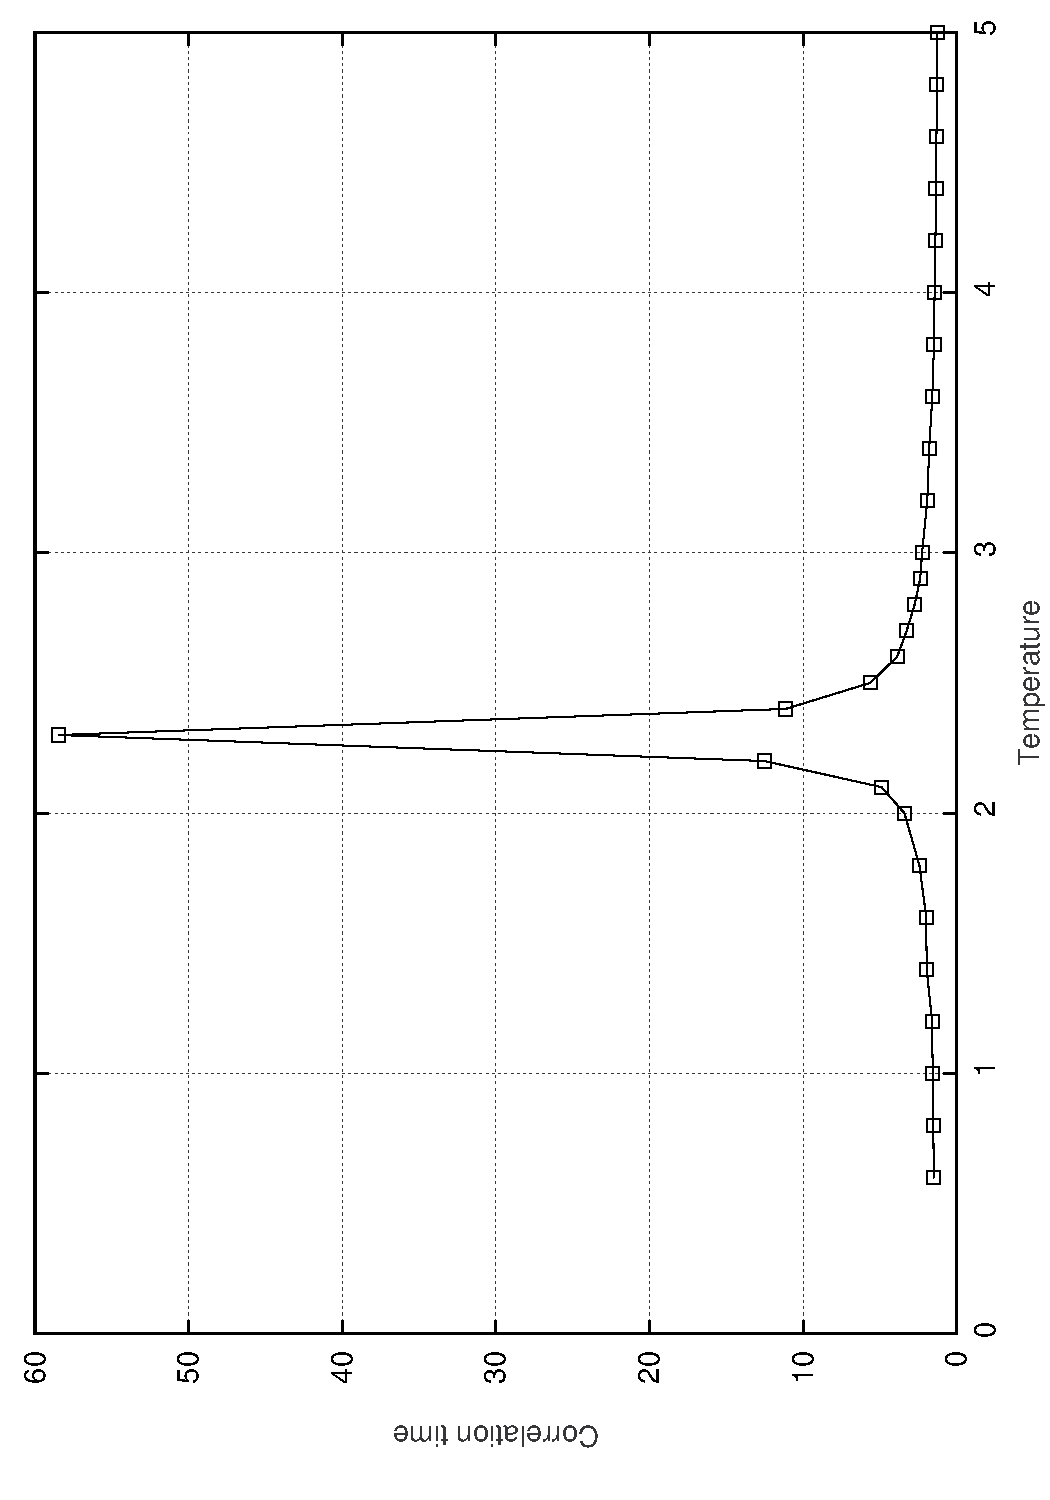
\includegraphics[angle=270, width=0.6\textwidth]{images/ctimes}
	\caption{{\footnotesize Gráfico de $\tau(T')$ para o modelo de Ising, onde T' é a temperatura reduzida ($T'\equiv\frac{k_b T}{J}$), com os pontos experimentais ligados por uma linha. A estimativa do tempo foi obtida após equilibrar o sistema com 10000 MCS (passos de monte carlo), calculando a função de autocorrelação (eq.7) e integrando-a, assumindo a forma exponencial já referida.}} 
	\label{fig:1}
\end{figure}
\end{frame}

\begin{frame}
\frametitle{\insertsection \\ {\small \insertsubsection}}
\begin{center}
\only<1>
{
\tiny $T=1.5$

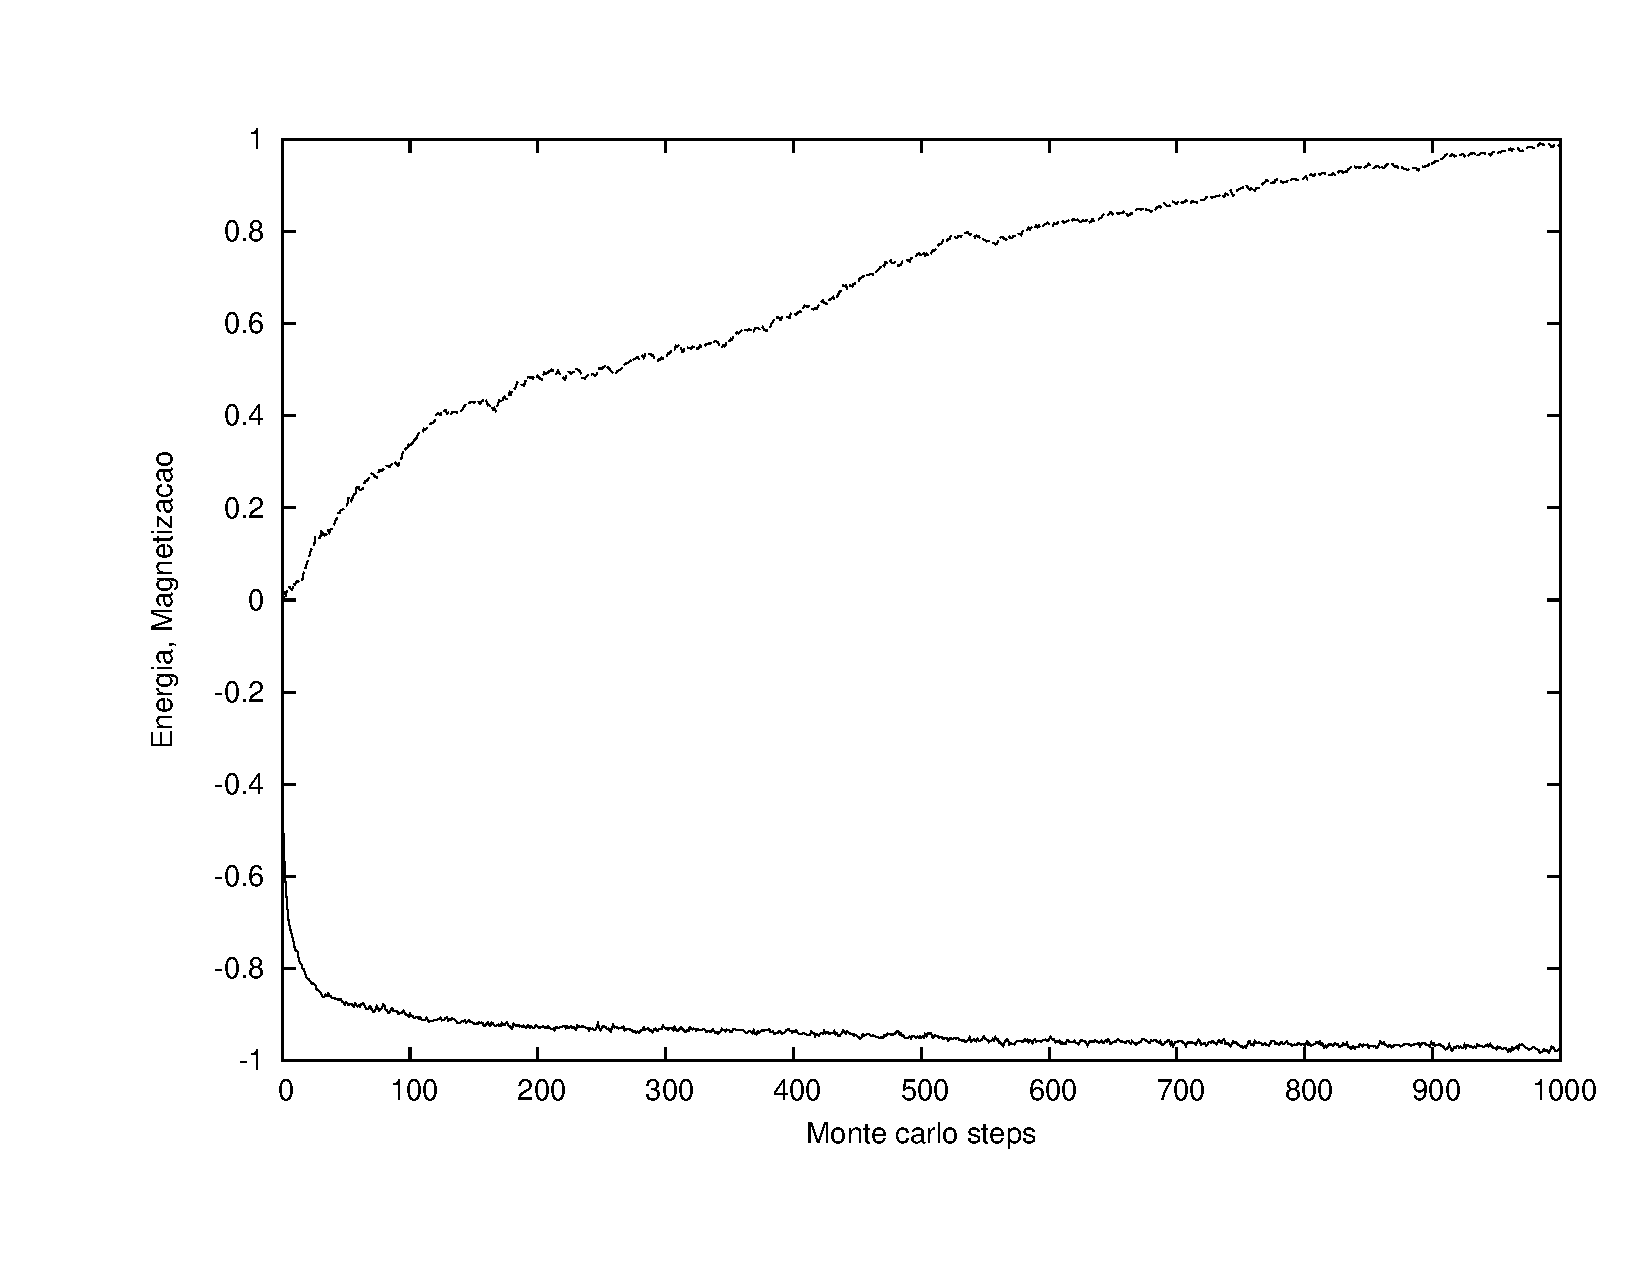
\includegraphics[angle=0, width=0.6\textwidth, clip, trim = 1cm 2cm 1cm 2cm]{images/vars15}
}
\only<2>
{
\tiny $T=2$

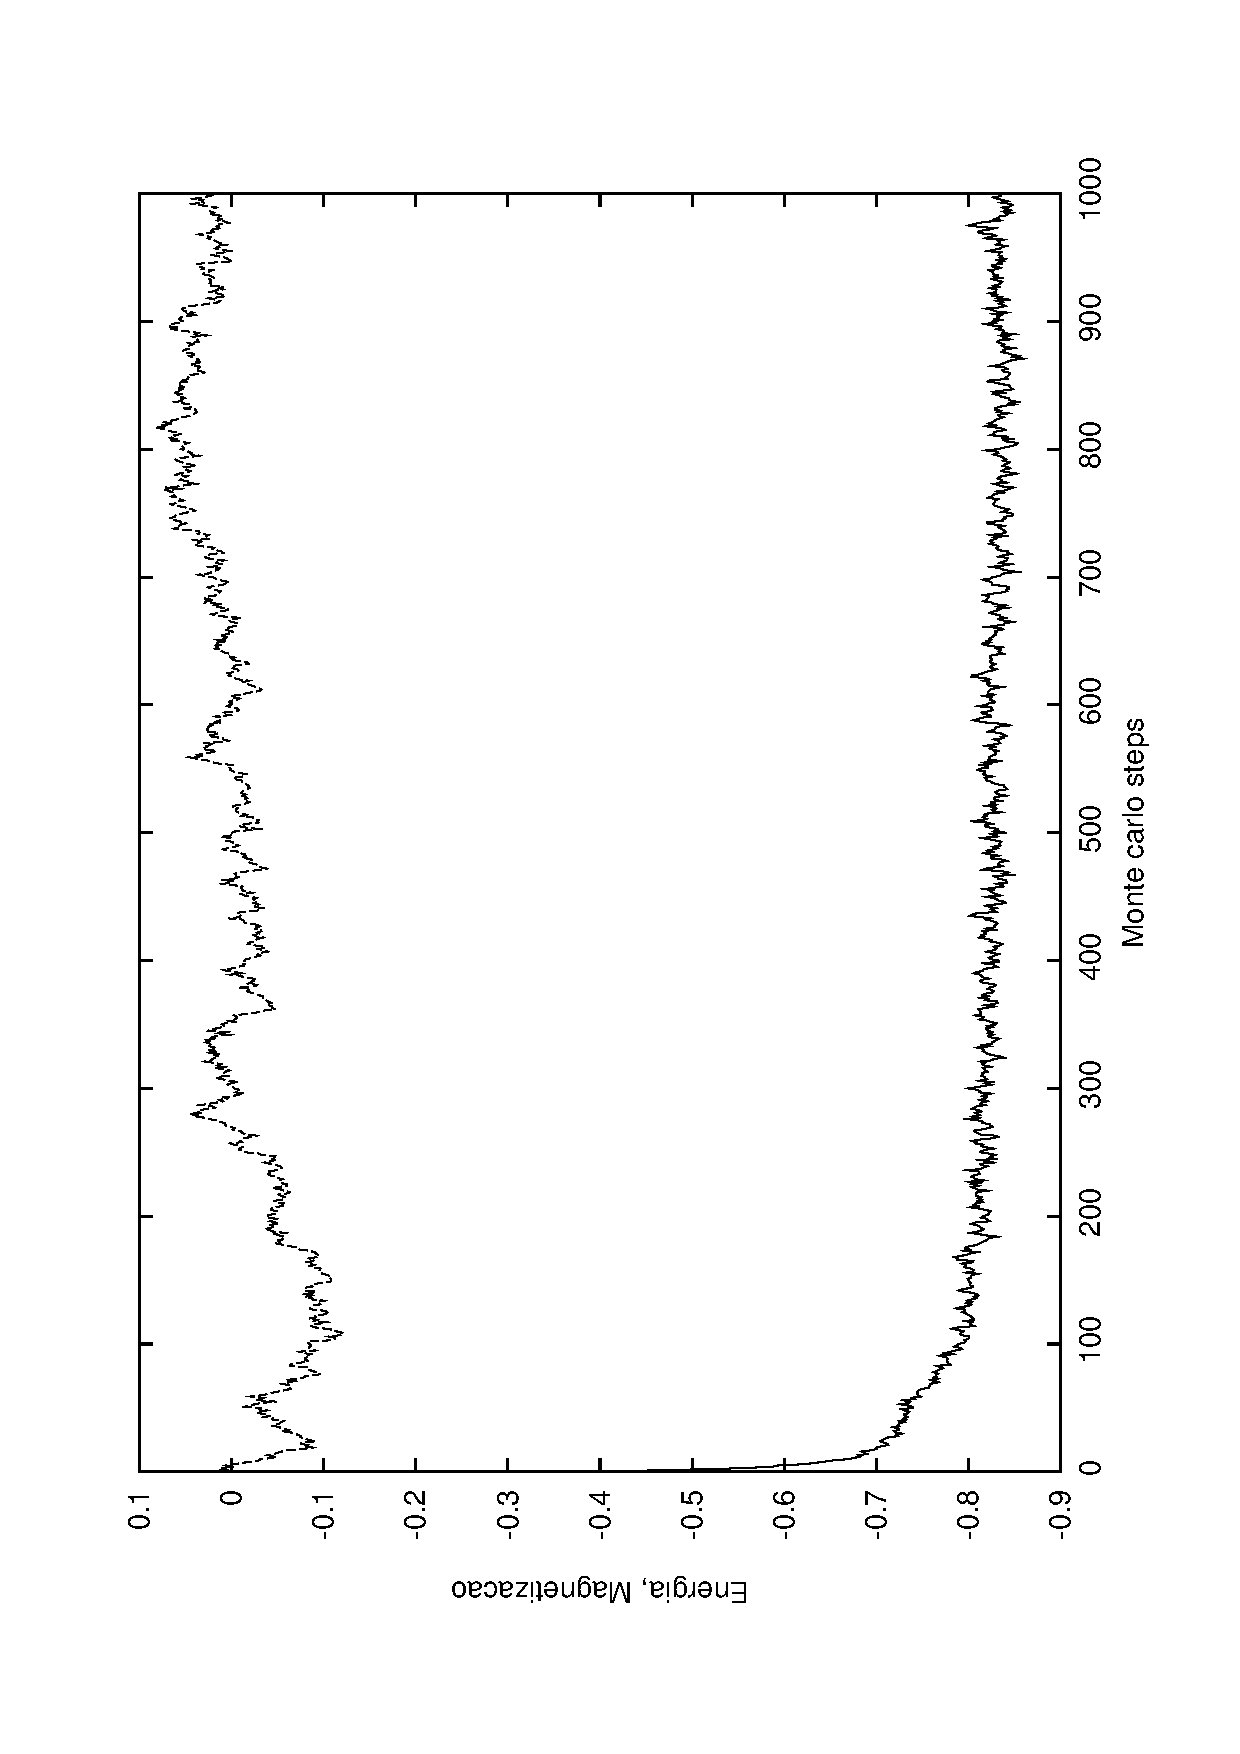
\includegraphics[angle=0, width=0.6\textwidth, clip, trim = 1cm 2cm 1cm 2cm]{images/vars2}
}
\only<3>
{
\tiny $T=2.3$

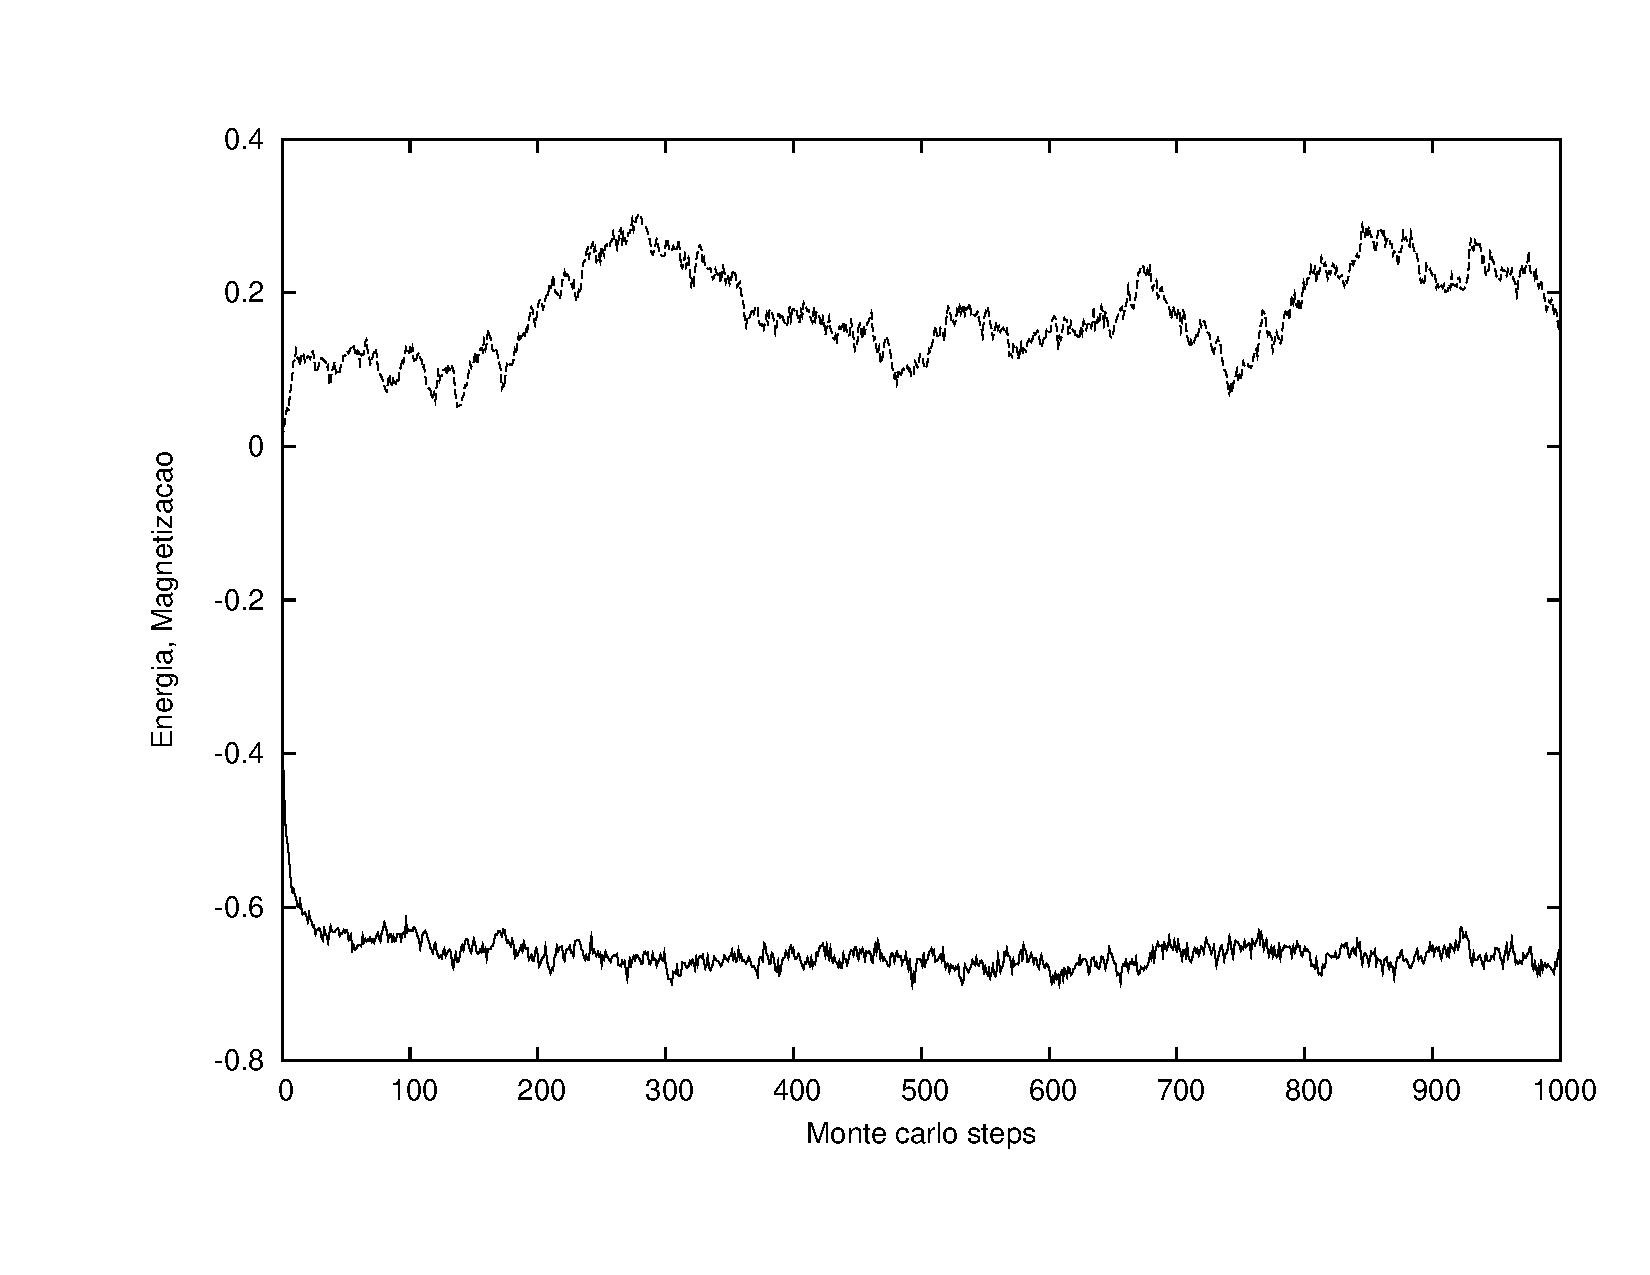
\includegraphics[angle=0, width=0.6\textwidth, clip, trim = 1cm 2cm 1cm 2cm]{images/vars23}
}
\only<4>
{
\tiny $T=3.2$

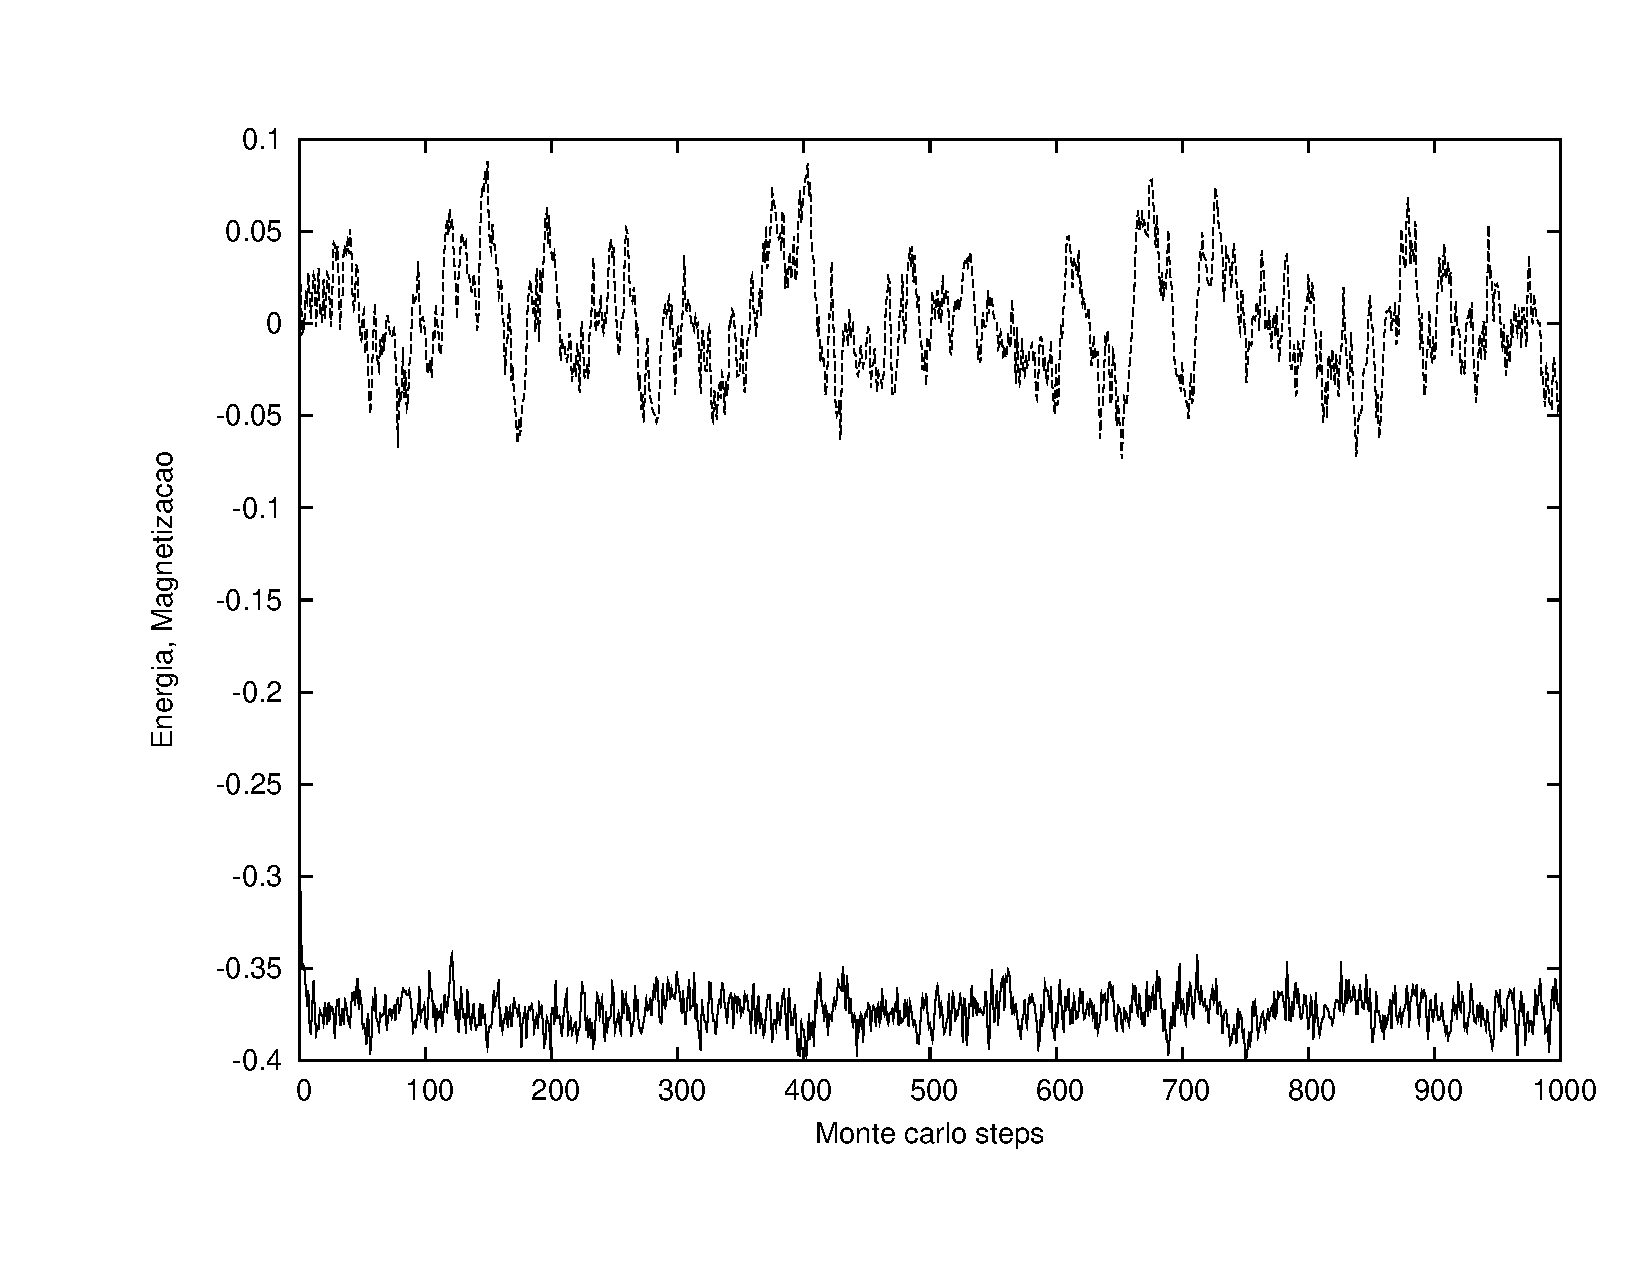
\includegraphics[angle=0, width=0.6\textwidth, clip, trim = 1cm 2cm 1cm 2cm]{images/vars32}
}
\end{center}

{\footnotesize Evolução da energia e magnetização para várias temperaturas. Os gráficos demonstram o sistema a evoluir para o equilíbrio, minimizando a energia. As quantidades apresentadas são novamente reduzidas, com $m =\frac{M}{N}$ onde $M=\sum_i s_i$ e $E'=\frac{E}{2N}$. }

\end{frame}

\subsection{Modelo de Agregação linear a 2D}

\subsubsection{Visualização}

\begin{frame}
\frametitle{\insertsection \\ {\small \insertsubsection}}
\begin{figure}
	\centering
%\only<1>{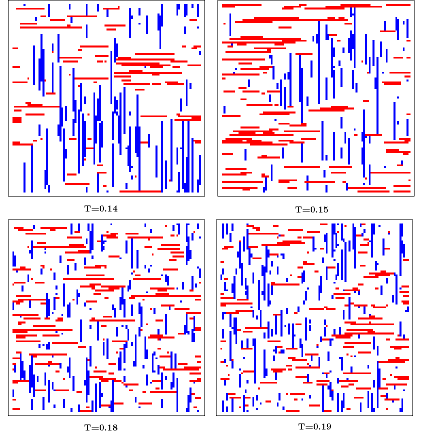
\includegraphics[width=0.5\textwidth, clip, trim = 0cm 32cm 15cm 0cm]{images/rods2d}}
%\only<2>{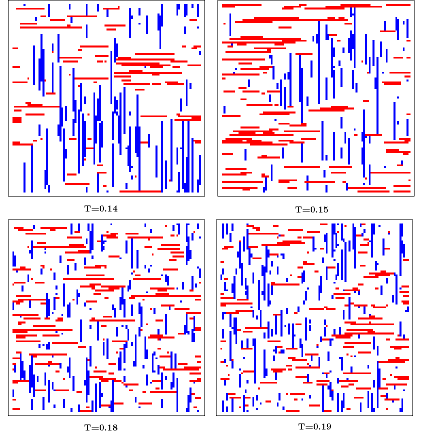
\includegraphics[width=0.5\textwidth, clip, trim = 15cm 32cm 0cm 0cm]{images/rods2d}}
%\only<3>{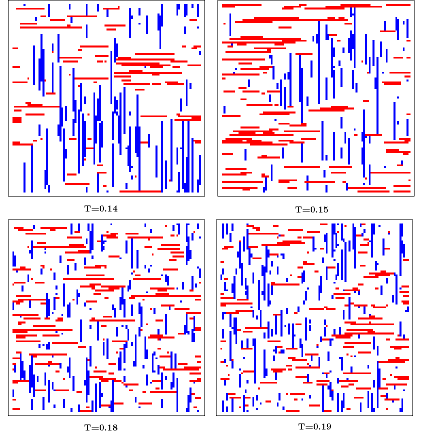
\includegraphics[width=0.5\textwidth, clip, trim = 0cm 16.5cm 15cm 15cm]{images/rods2d}}
%\only<4>{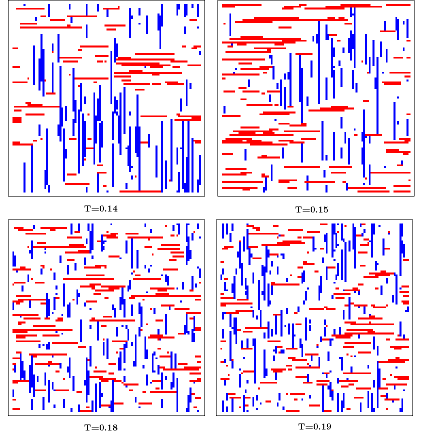
\includegraphics[width=0.5\textwidth, clip, trim = 15cm 16.5cm 0cm 15cm]{images/rods2d}}
%\only<5>{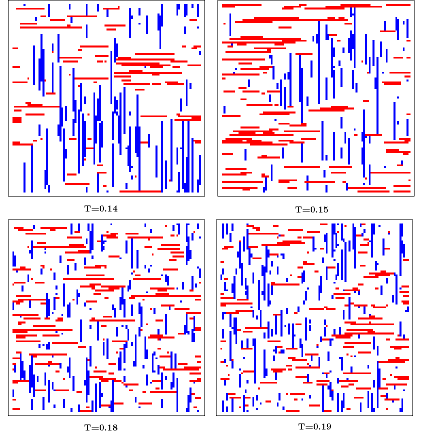
\includegraphics[width=0.5\textwidth, clip, trim = 0cm 0cm 15cm 31cm]{images/rods2d}}
%\only<6>{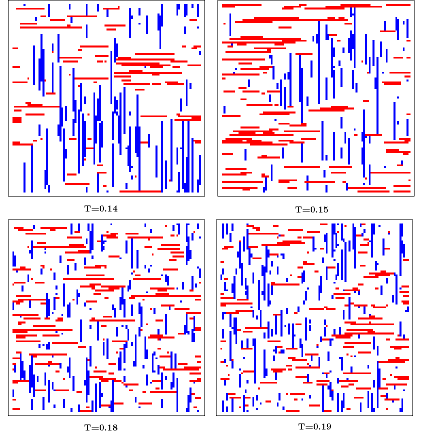
\includegraphics[width=0.5\textwidth, clip, trim = 15cm 0cm 0cm 31cm]{images/rods2d}}
	\caption{{\footnotesize Visualização do sistema 2D para $T \in [1.4,1.9]$, onde as partículas são representadas por quadrados vermelhos e azuis, respectivamente horizontais e verticais.}}     
	\label{fig:2}
\end{figure}
\end{frame}

\subsubsection{Resultados experimentais}

\begin{frame}
\frametitle{\insertsection \\ {\small \insertsubsection}}
\begin{figure}
	\centering
		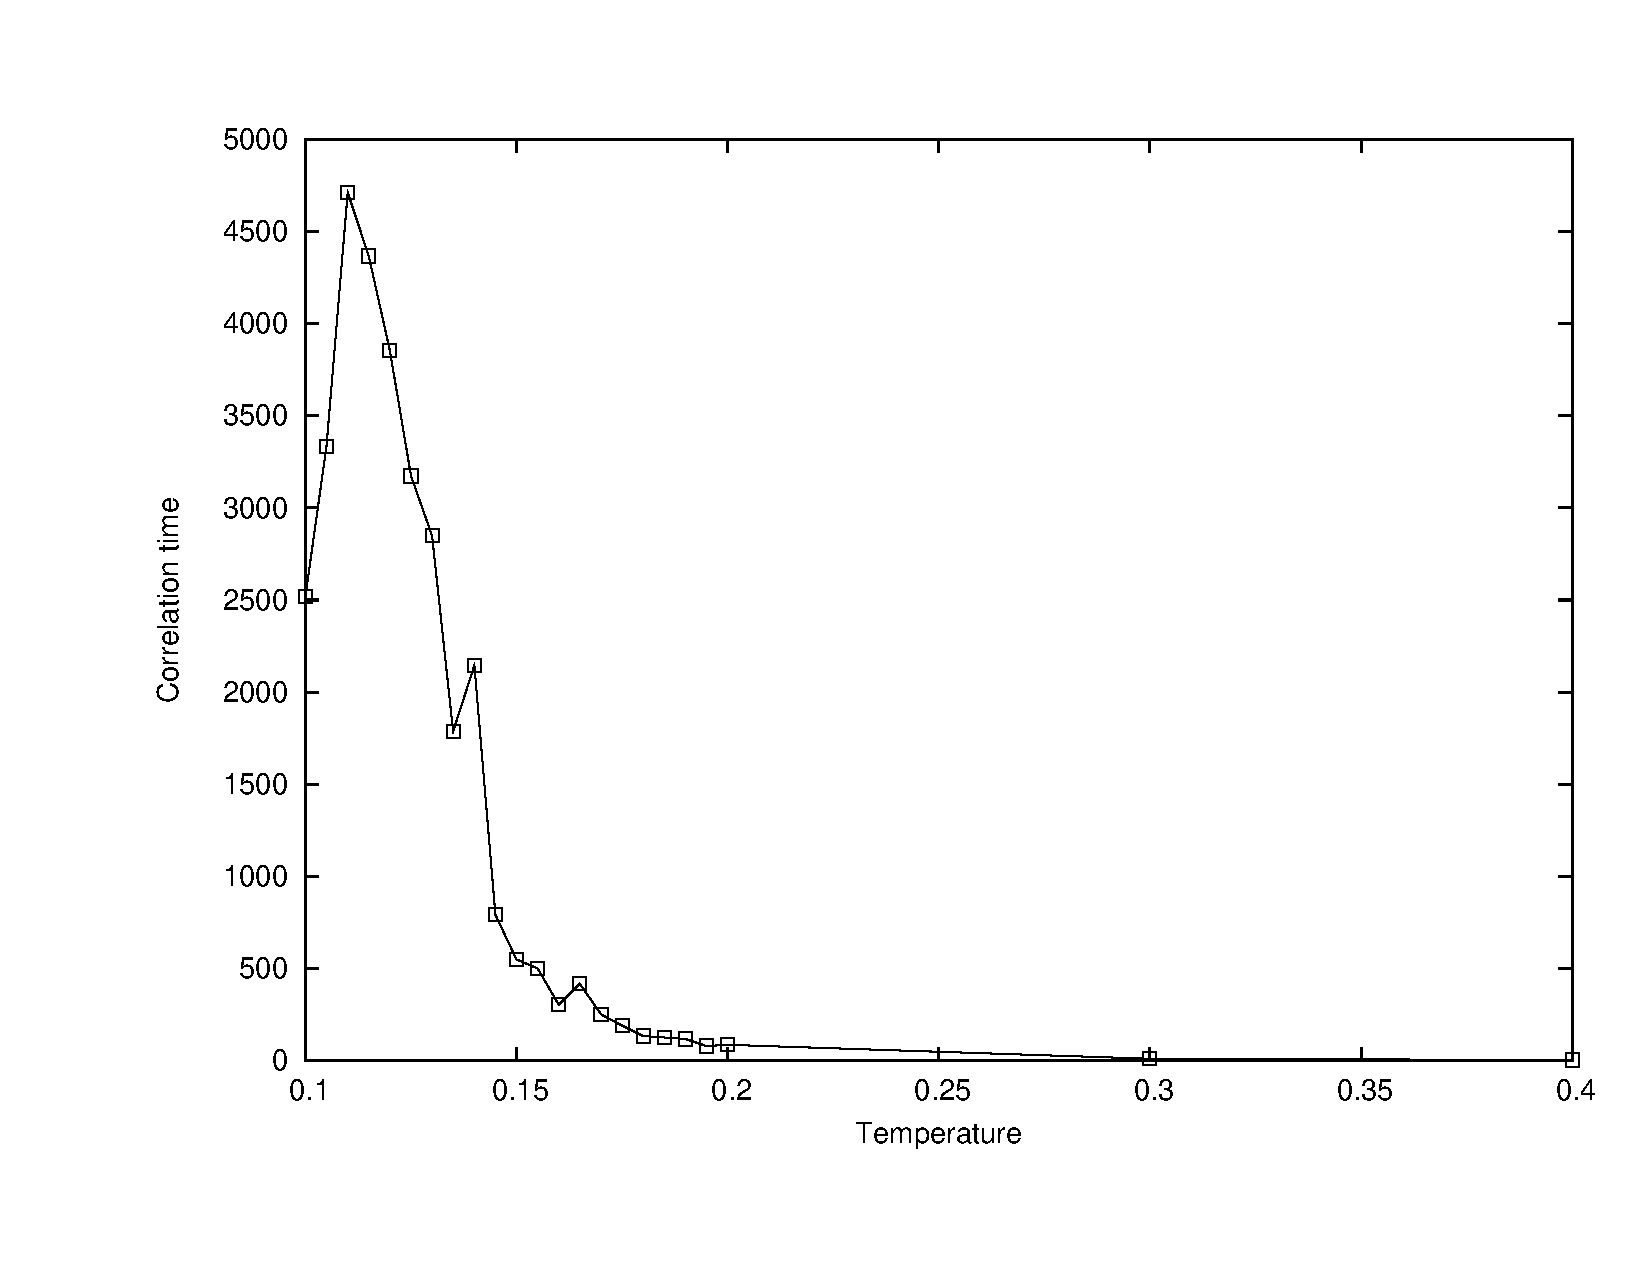
\includegraphics[width=0.5\textwidth]{images/ctimesr2d}
	\caption{{\footnotesize Gráfico de $\tau(T')$ para o modelo de agregação a 2D, onde T' é a temperatura reduzida ($T'\equiv\frac{k_b T}{\epsilon}$), com os pontos experimentais ligados por uma linha. A estimativa do tempo foi obtida após equilibrar o sistema com 100000 MCS (passos de monte carlo), calculando a função de autocorrelação (eq.7) e integrando-a, assumindo a forma exponencial já referida.}}
	\label{fig:3}
\end{figure}
\end{frame}

\begin{frame}
\frametitle{\insertsection \\ {\small \insertsubsection}}
\begin{figure}
	\centering
		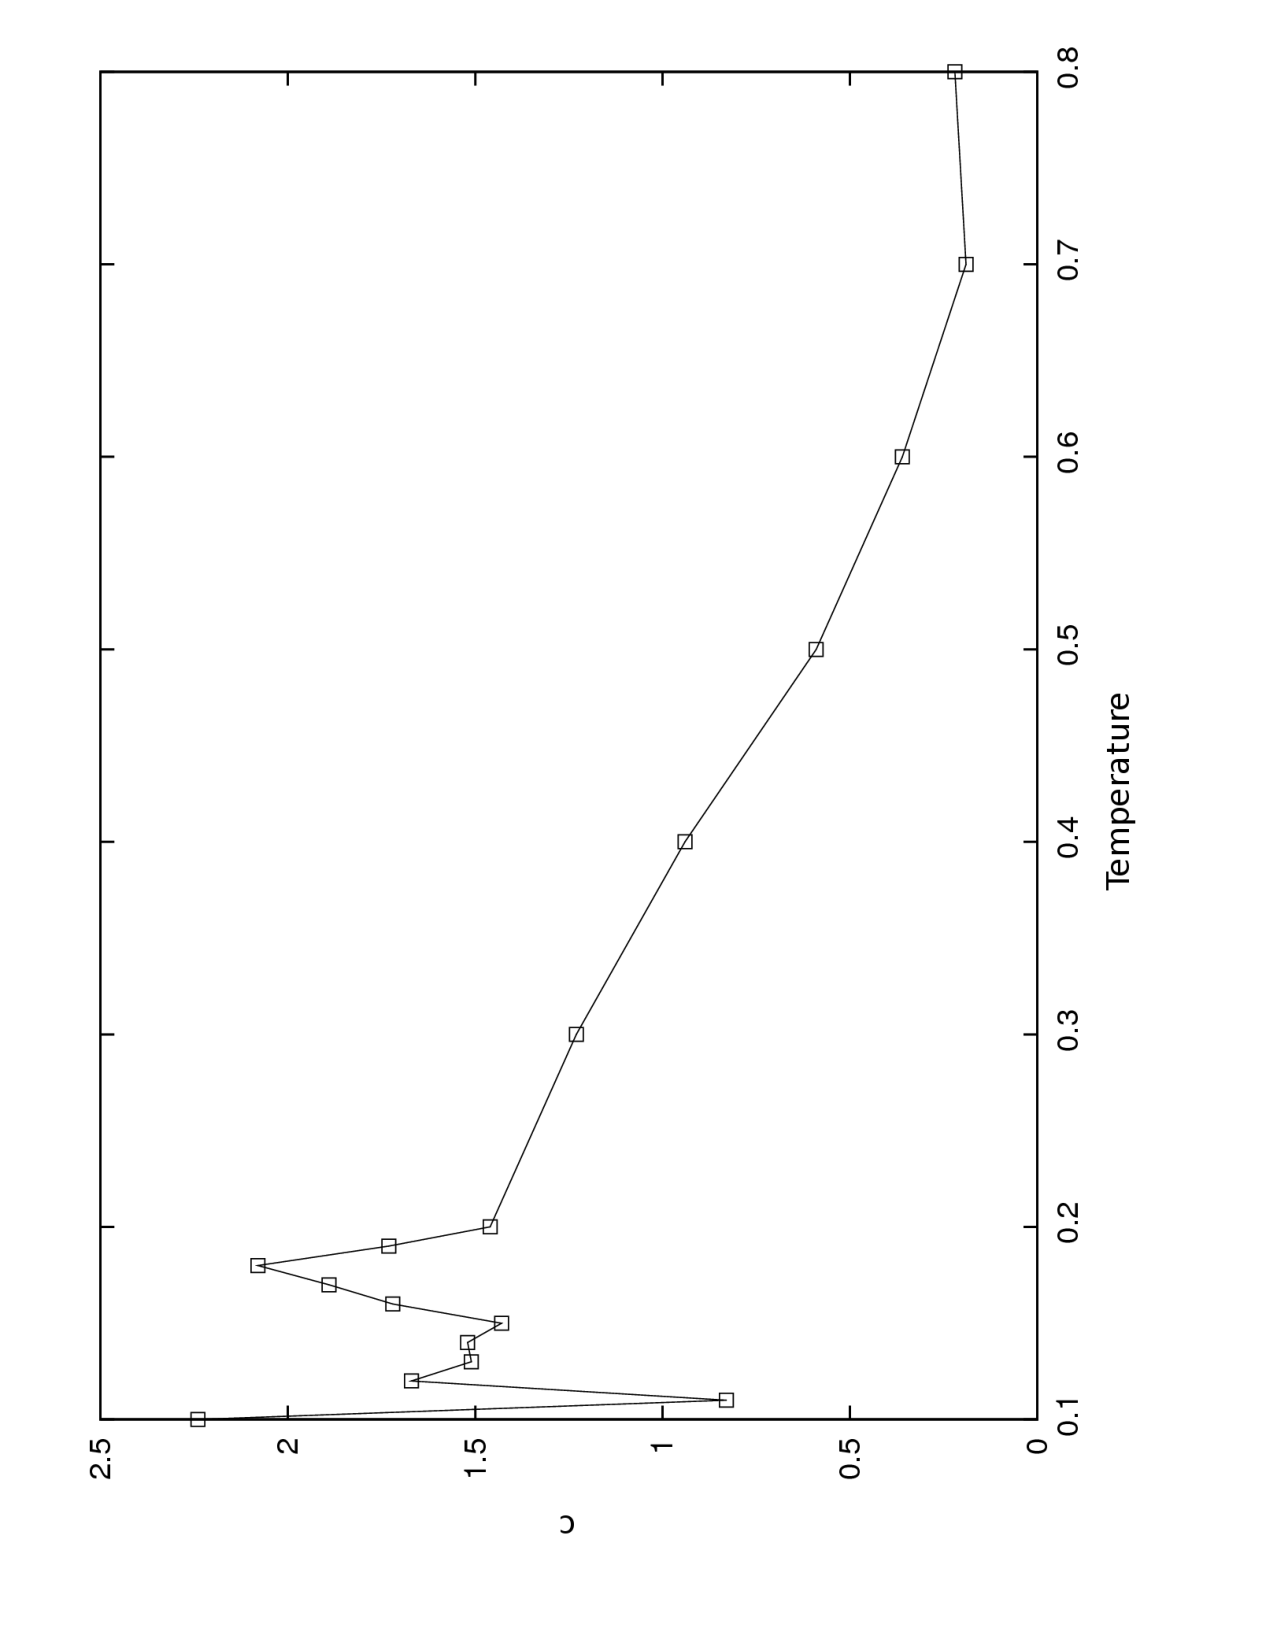
\includegraphics[angle=-90, clip, trim = 1cm 2cm 1cm 1cm, width=0.6\textwidth]{images/c2d}
	\caption{{\footnotesize Calor específico $c$ para o modelo de agregação a 2D com $\rho = 0.2$, calculado após equilibrar o sistema esperando 100000 MCS e fazendo 20 medições da energia a cada 2 tempos de correlação, calculando então as suas flutuações.}}
	\label{fig:4}
\end{figure}
\end{frame}

\begin{frame}
\frametitle{\insertsection \\ {\small \insertsubsection}}
\begin{figure}
	\centering
		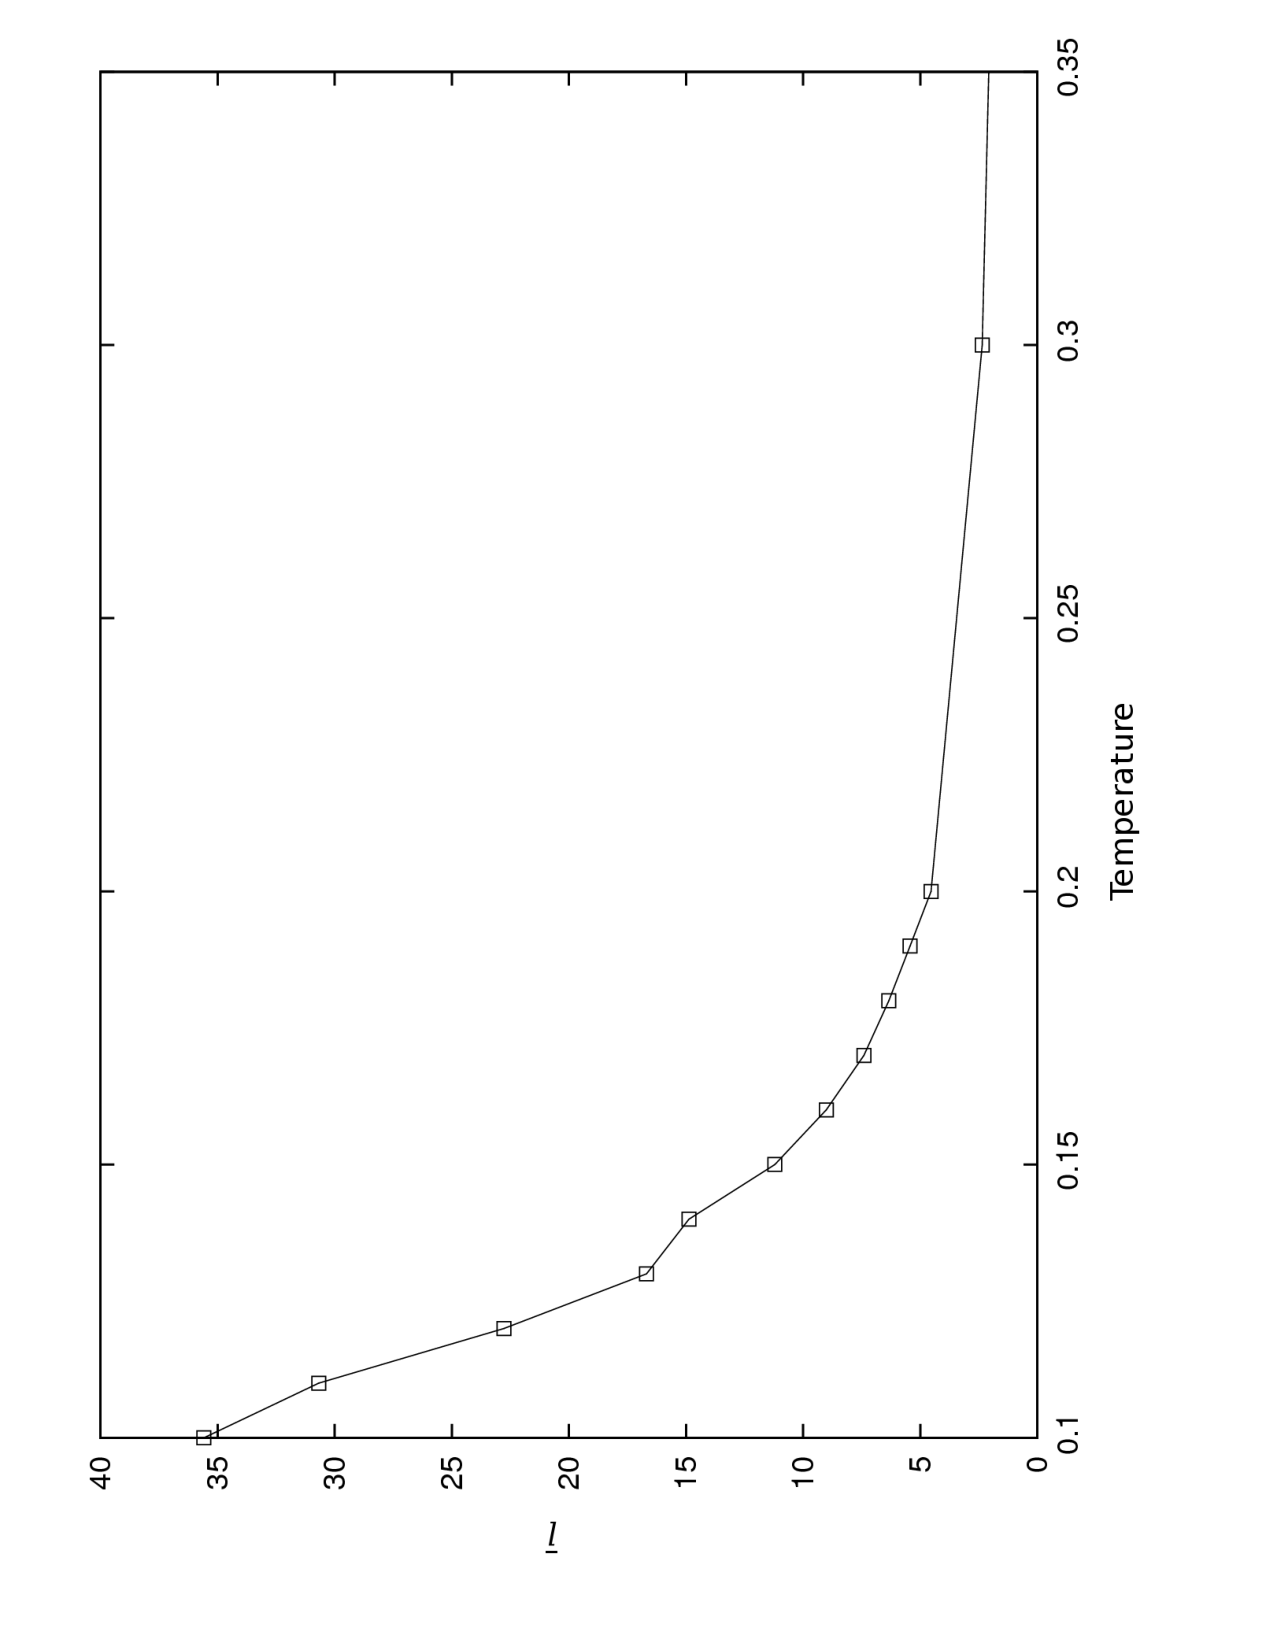
\includegraphics[angle=-90, clip, trim = 1cm 2cm 1cm 1cm, width=0.6\textwidth]{images/lav2d}
	\caption{{\footnotesize Comprimento médio das cadeias $\bar{l}$ para o modelo de agregação a 2D com $\rho = 0.2$, calculado após equilibrar o sistema esperando 100000 MCS e fazendo 20 medições de $\bar{l}$ a cada 2 tempos de correlação, calculando então a sua média.}}
	\label{fig:5}
\end{figure}
\end{frame}

\begin{frame}
\frametitle{\insertsection \\ {\small \insertsubsection}}
\begin{figure}
	\centering
		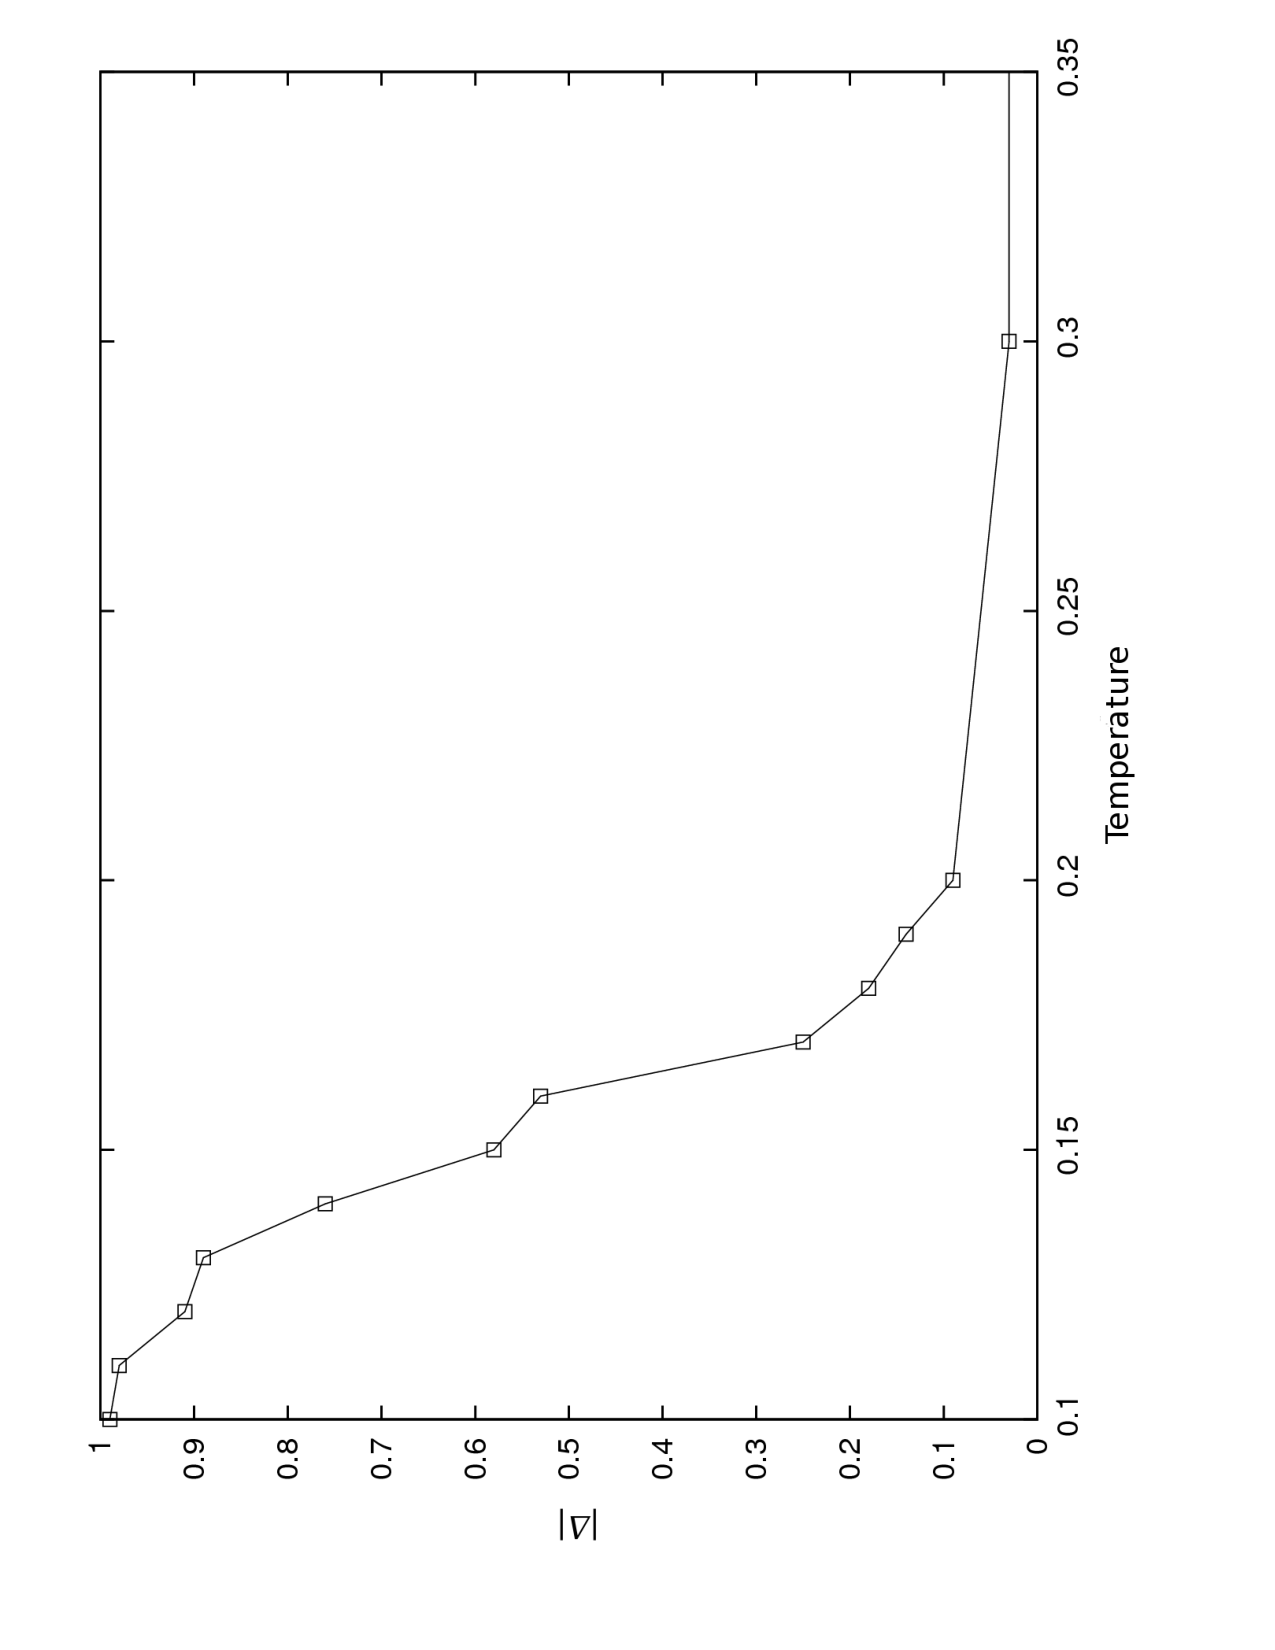
\includegraphics[angle=-90, clip, trim = 1cm 2cm 1cm 1cm, width=0.6\textwidth]{images/delta2d}
	\caption{{\footnotesize Parâmetro de ordem reduzido $|\Delta|$ para o modelo de agregação a 2D com $\rho = 0.2$. O parâmetro foi calculado após equilibrar o sistema esperando 100000 MCS e fazendo 20 medições de $|\Delta|$ a cada 2 tempos de correlação, calculando então a sua média.}}
	\label{fig:6}
\end{figure}
\end{frame}

\subsection{Modelo de Agregação linear a 3D}
\subsubsection{Resultados experimentais: $\rho=0.1$}

\begin{frame}
\frametitle{\insertsection \\ {\small \insertsubsection}}
\begin{figure}
	\centering
		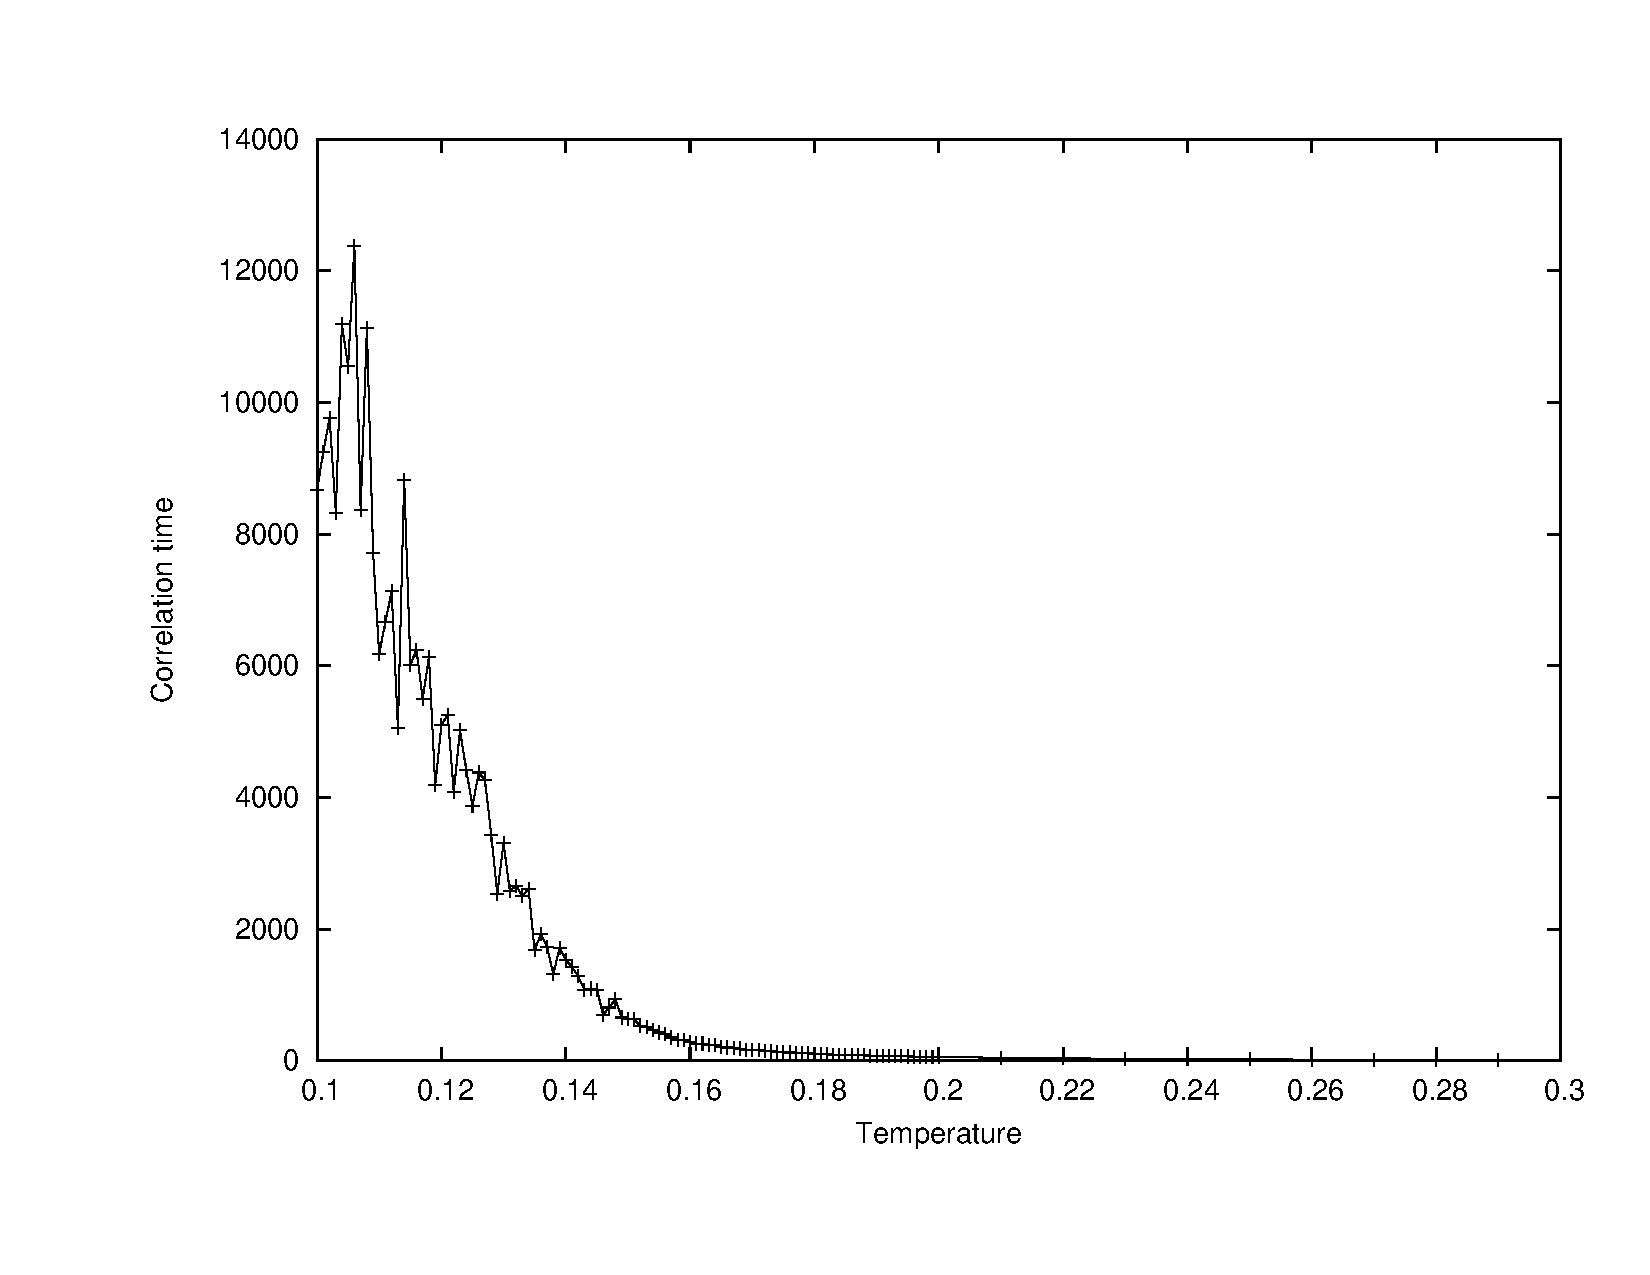
\includegraphics[width=0.5\textwidth, clip, trim = 1.7cm 1.5cm 1cm 1cm]{images/ctimes1}
	\caption{{\footnotesize Gráfico de $\tau(T')$ para o modelo de agregação a 3D, onde T' é a temperatura reduzida ($T'\equiv\frac{k_b T}{\varepsilon}$), para $\rho = 0.1$, com os pontos experimentais ligados por uma linha. A estimativa do tempo foi obtida após equilibrar o sistema com 500000 MCS (passos de monte carlo), calculando a função de autocorrelação (eq.7) e integrando-a, assumindo a forma exponencial já referida.}}
	\label{fig:7}
\end{figure}
\end{frame}

\begin{frame}
\frametitle{\insertsection \\ {\small \insertsubsection}}
\begin{figure}
	\centering
		\includegraphics[width=0.5\textwidth, clip, trim = 1.7cm 1.5cm 1cm 1cm]{images/0.1/c}
	\caption{{\footnotesize Calor específico $c$ para $\rho = 0.1$, calculado após equilibrar o sistema esperando 500000 MCS e fazendo 20 medições da energia a cada 2 tempos de correlação, calculando então as suas flutuações.}}
	\label{fig:8}
\end{figure}
\end{frame}

\begin{frame}
\frametitle{\insertsection \\ {\small \insertsubsection}}
\begin{figure}
	\centering
		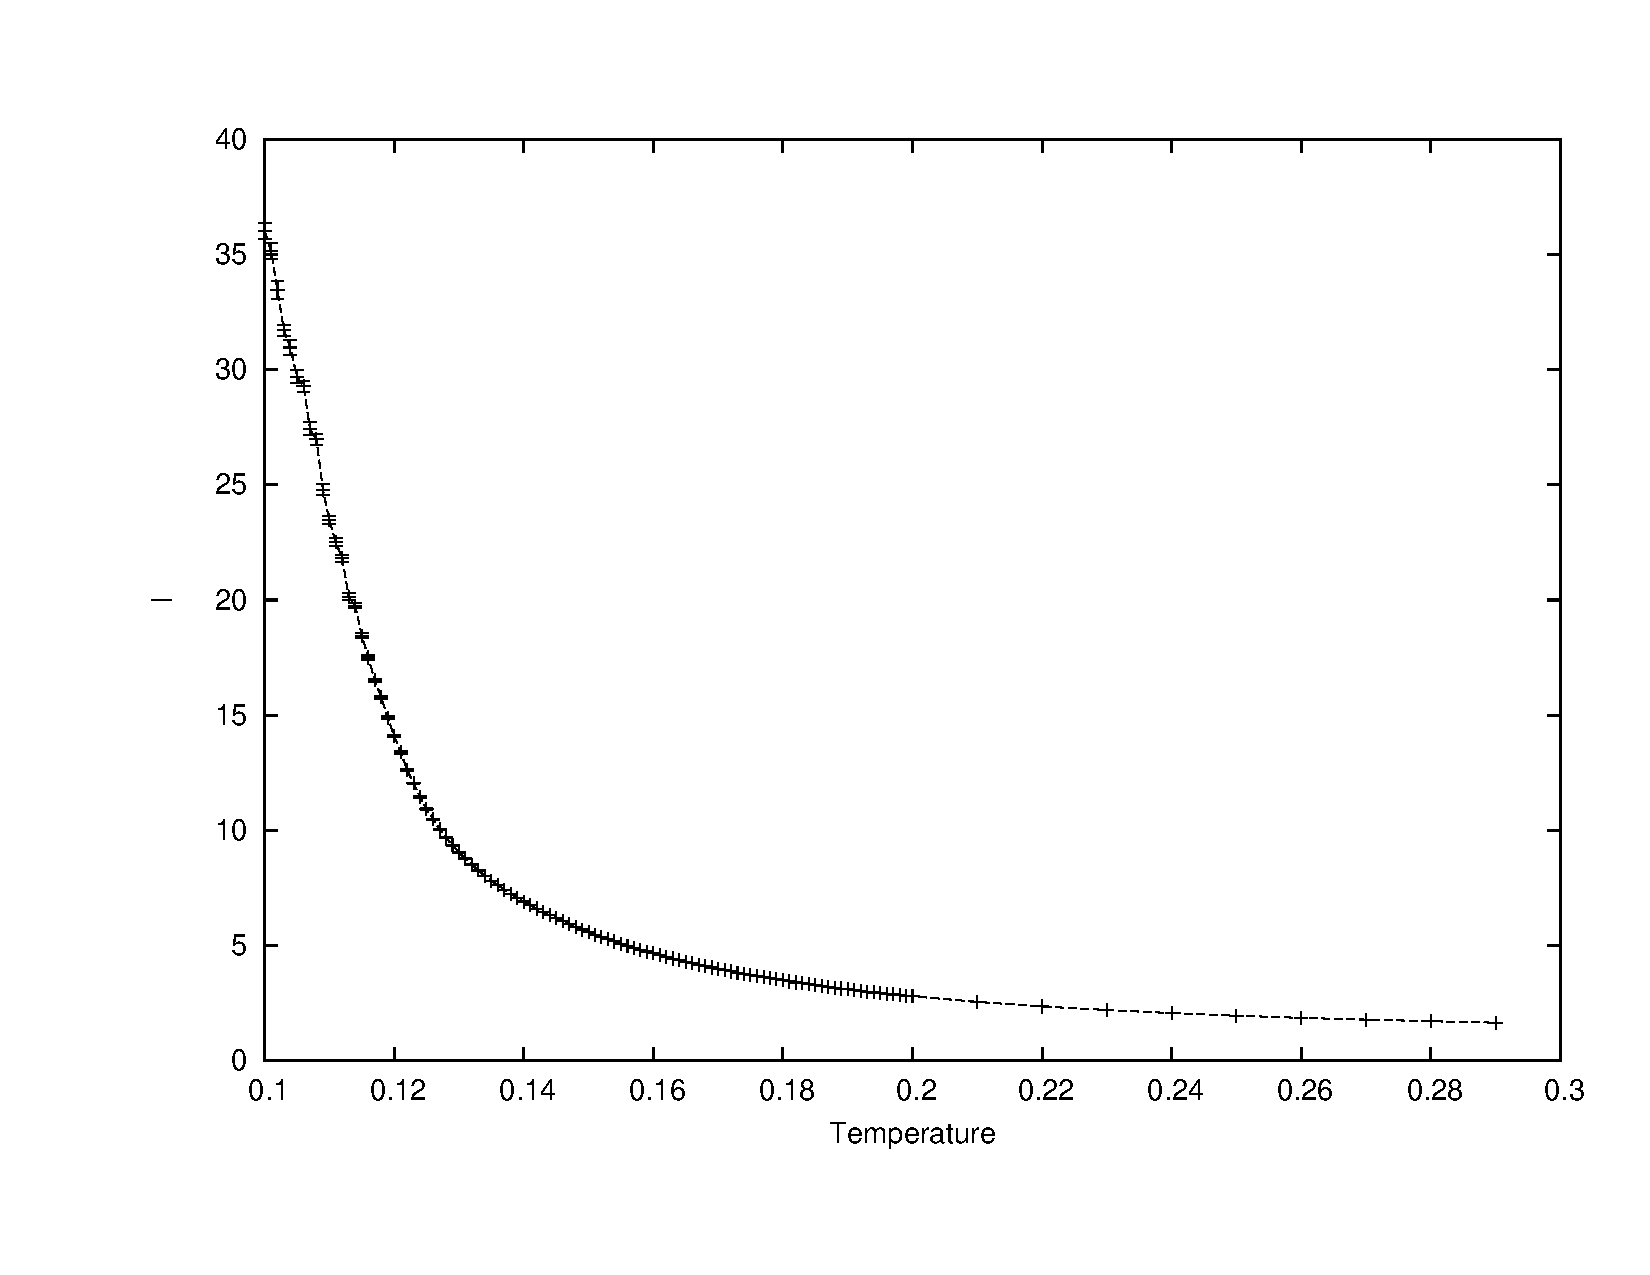
\includegraphics[width=0.5\textwidth, clip, trim = 1.7cm 1.5cm 1cm 1cm]{images/0.1/l}
	\caption{{\footnotesize Comprimento médio das cadeias $\bar{l}$ para $\rho = 0.1$, calculado após equilibrar o sistema esperando 500000 MCS e fazendo 20 medições de $\bar{l}$ a cada 2 tempos de correlação, calculando então a sua média.}}
	\label{fig:9}
\end{figure}
\end{frame}

\begin{frame}
\frametitle{\insertsection \\ {\small \insertsubsection}}
\begin{figure}
	\centering
		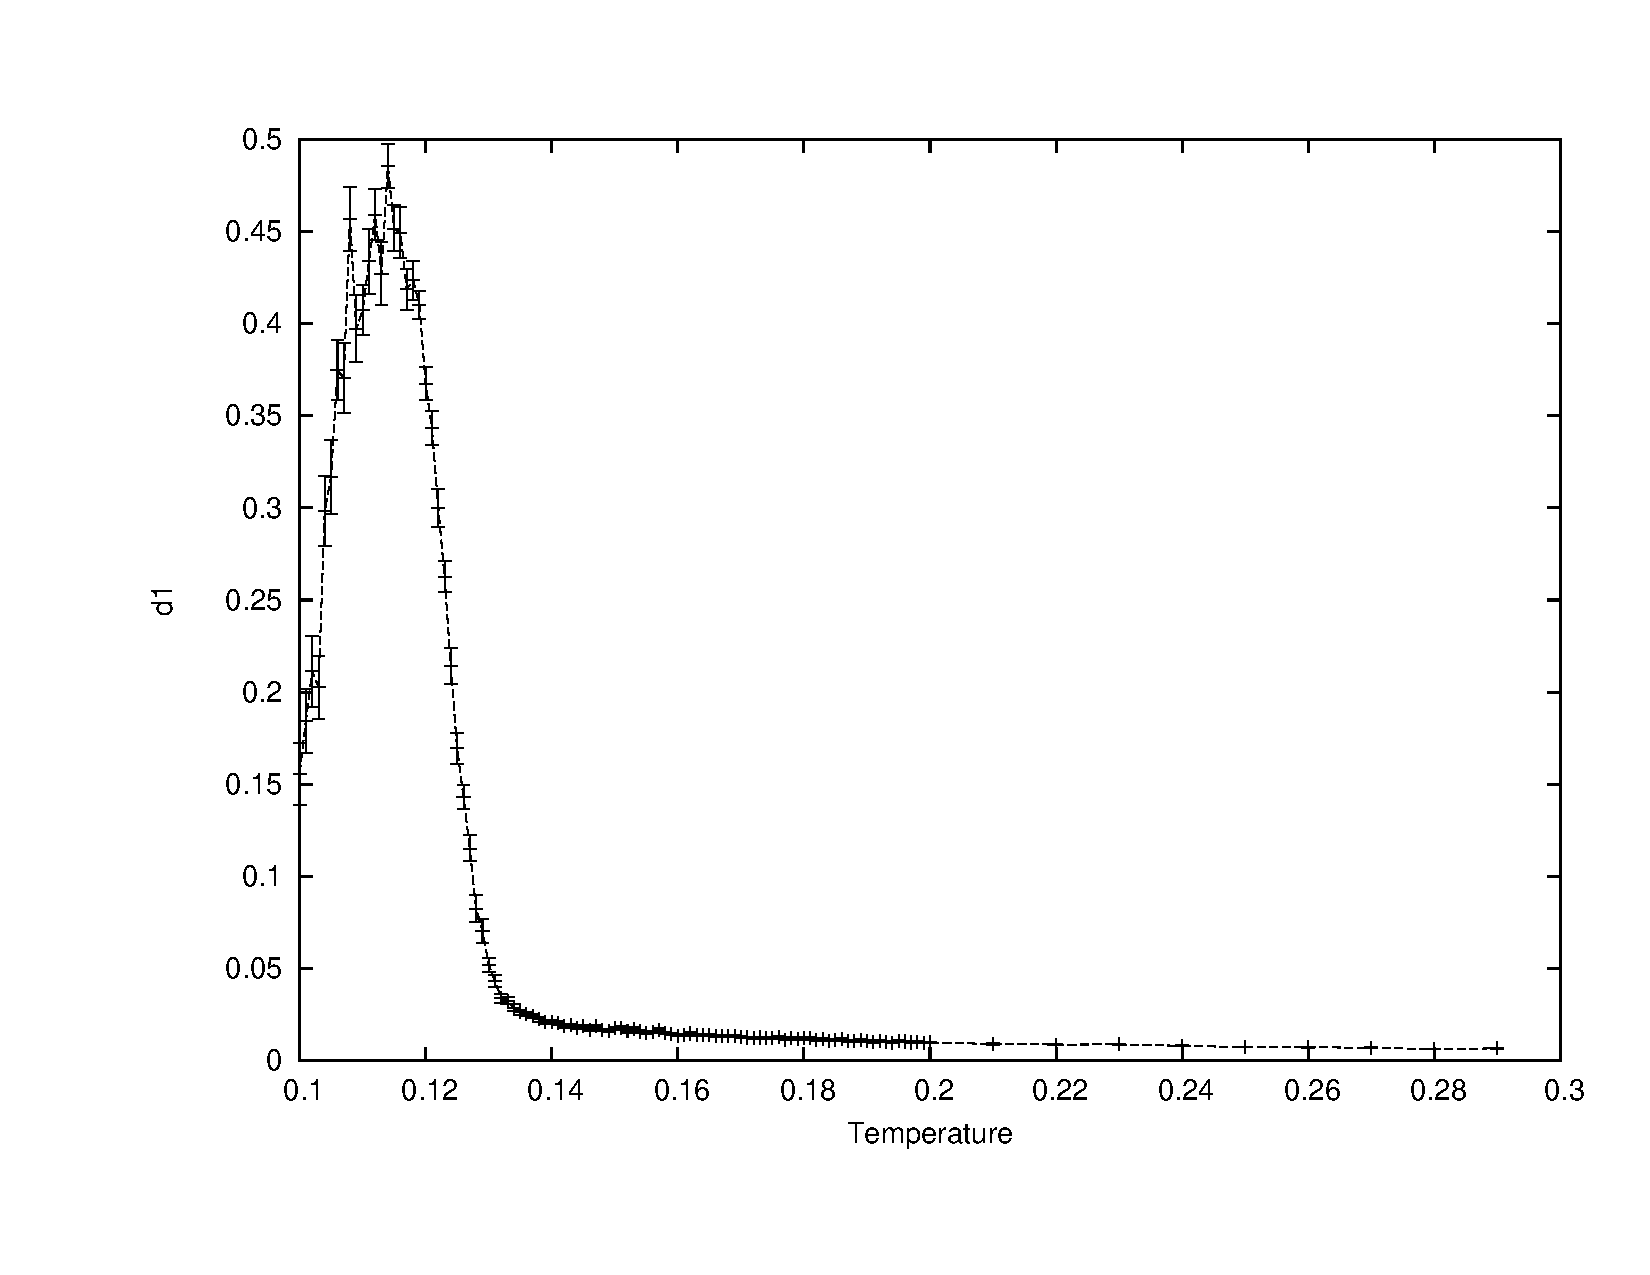
\includegraphics[width=0.5\textwidth, clip, trim = 1.7cm 1.5cm 1cm 1cm]{images/0.1/d1}
	\caption{{\footnotesize Parâmetro de ordem reduzido $|\Delta_1|$ para $\rho = 0.1$, onde $N$ é o número total de partículas. O parâmetro foi calculado após equilibrar o sistema esperando 500000 MCS e fazendo 20 medições de $|\Delta_1|$ a cada 2 tempos de correlação, calculando então a sua média.}}
	\label{fig:10}
\end{figure}
\end{frame}

\begin{frame}
\frametitle{\insertsection \\ {\small \insertsubsection}}
\begin{figure}
	\centering
		\includegraphics[width=0.5\textwidth, clip, trim = 1.7cm 1.5cm 1cm 1cm]{images/0.1/d1f}
	\caption{{\footnotesize Flutuações do parâmetro de ordem reduzido $|\Delta_1|$ para $\rho = 0.1$, calculadas da mesma forma que c. Será em princípio possível ver a transição de fase determinando $T$ para a qual as flutuações tendem para infinito}}
	\label{fig:11}
\end{figure}
\end{frame}

\begin{frame}
\frametitle{\insertsection \\ {\small \insertsubsection}}
\begin{figure}
	\centering
		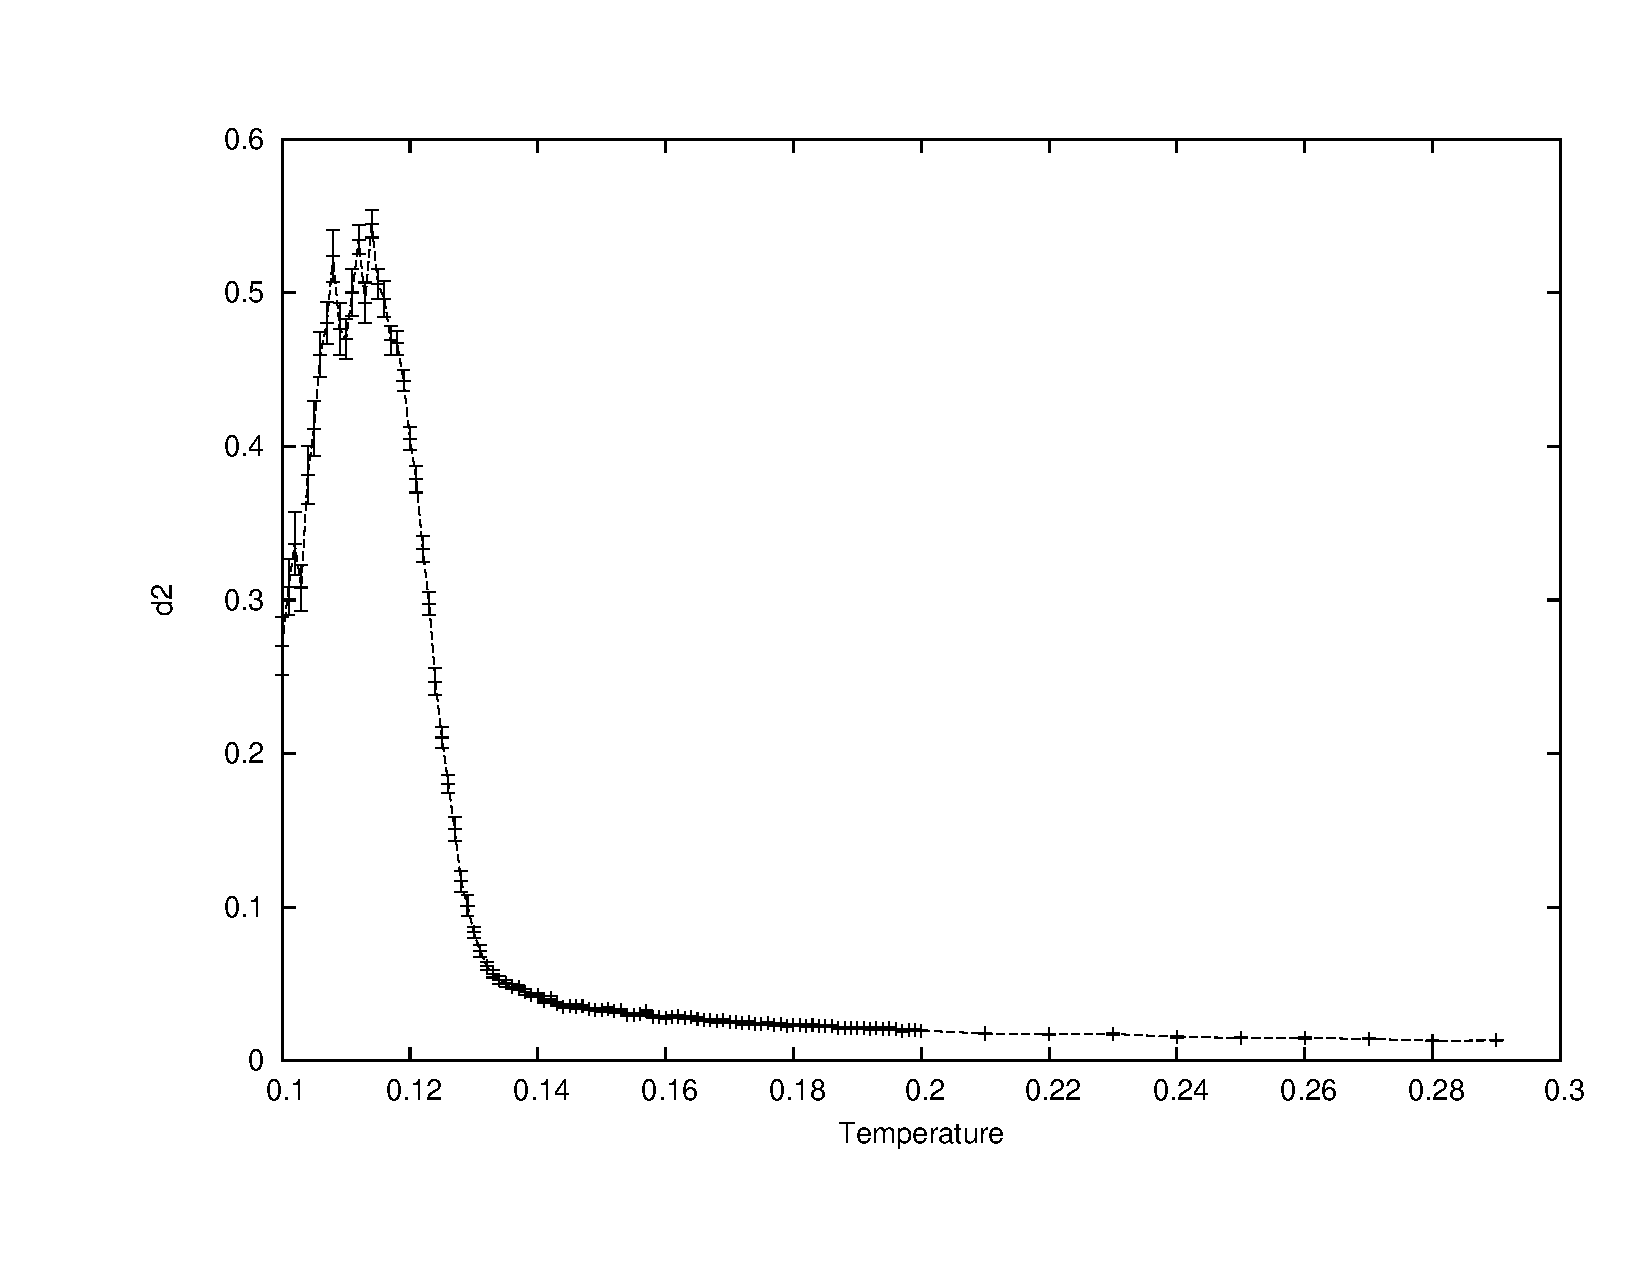
\includegraphics[width=0.5\textwidth, clip, trim = 1.7cm 1.5cm 1cm 1cm]{images/0.1/d2}
	\caption{{\footnotesize Parâmetro de ordem reduzido $|\Delta_2|$ para $\rho = 0.1$, onde $N$ é o número total de partículas. O parâmetro foi calculado após equilibrar o sistema esperando 500000 MCS e fazendo 20 medições de $|\Delta_2|$ a cada 2 tempos de correlação, calculando então a sua média.}}
	\label{fig:12}
\end{figure}
\end{frame}

\begin{frame}
\frametitle{\insertsection \\ {\small \insertsubsection}}
\begin{figure}
	\centering
		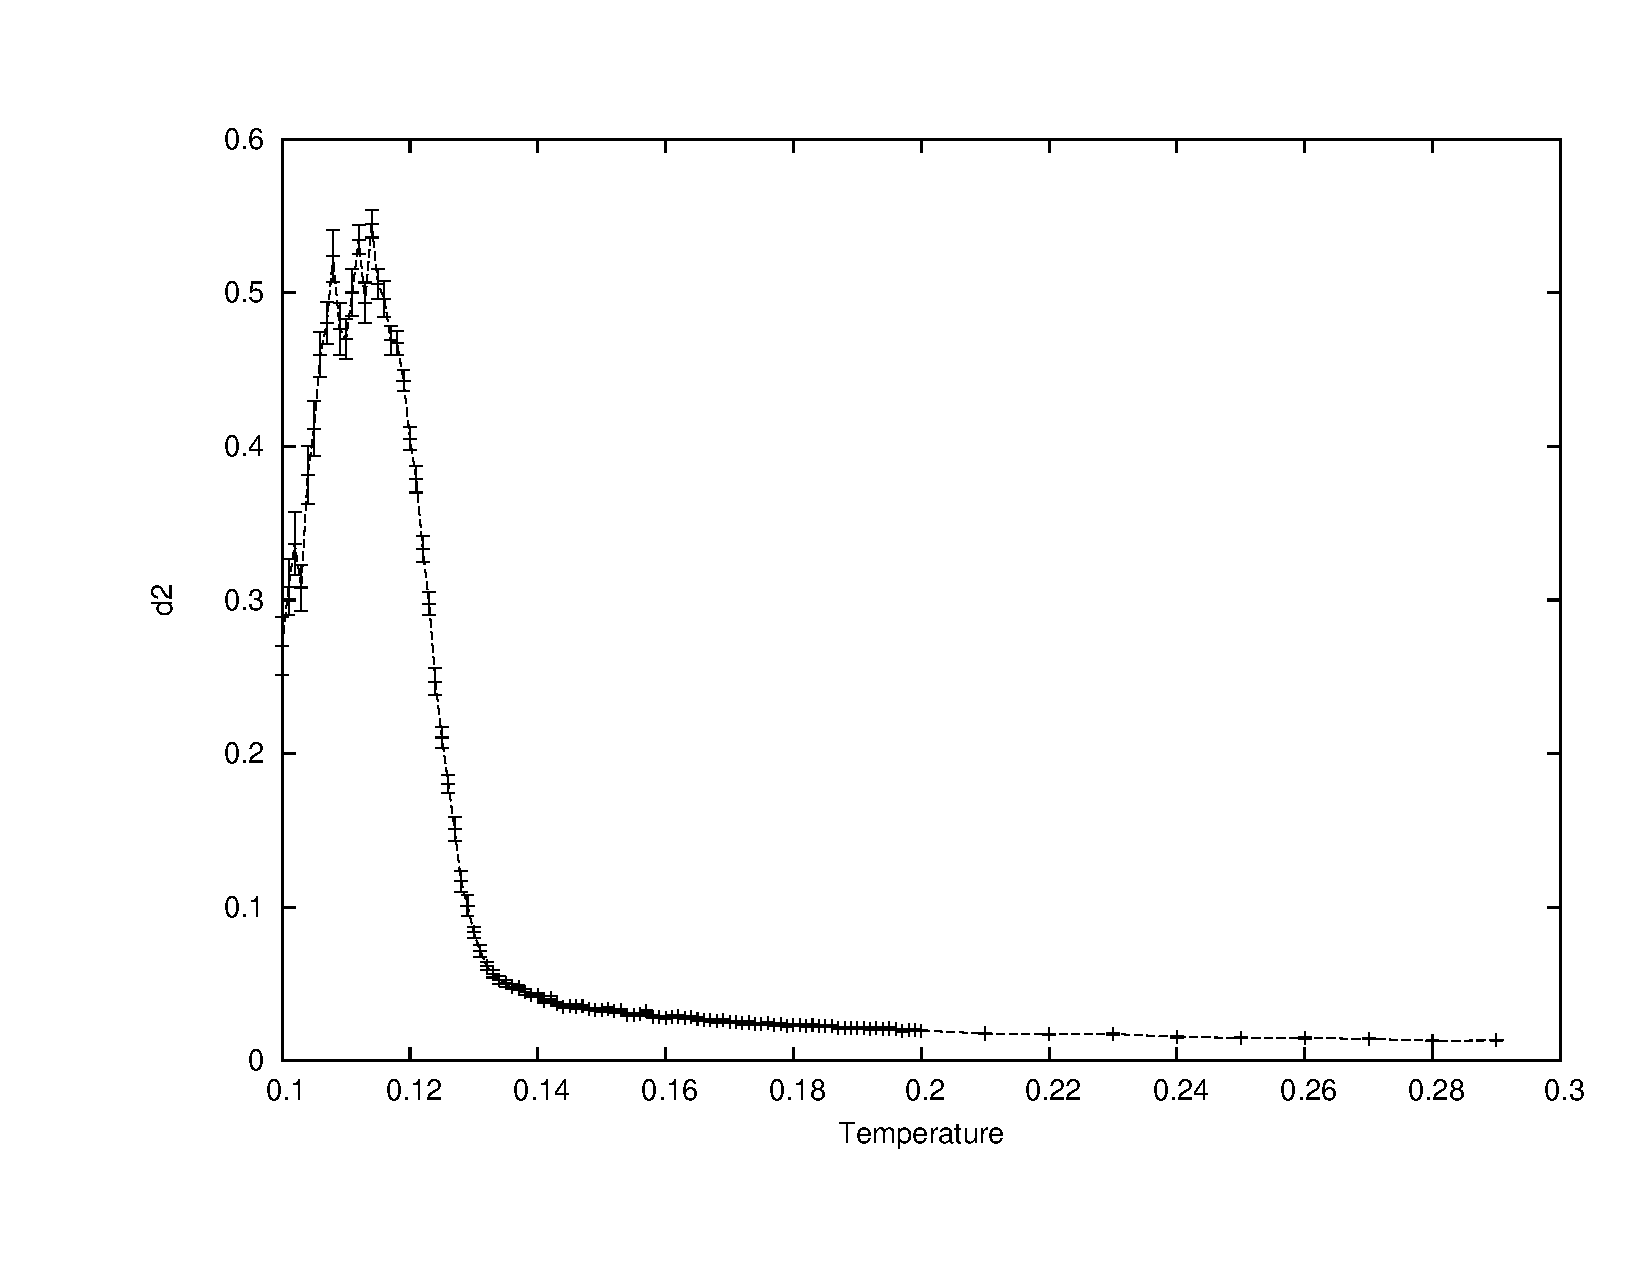
\includegraphics[width=0.5\textwidth, clip, trim = 1.7cm 1.5cm 1cm 1cm]{images/0.1/d2}
	\caption{{\footnotesize Flutuações do parâmetro de ordem reduzido $\frac{|\Delta_2|}{N}$ para $\rho = 0.1$, calculadas da mesma forma que c. Será em princípio possível ver a transição de fase determinando $T$ para a qual as flutuações tendem para infinito}}
	\label{fig:13}
\end{figure}
\end{frame}

\subsubsection{Resultados experimentais: $\rho=0.2$}

\begin{frame}
\frametitle{\insertsection \\ {\small \insertsubsection}}
\begin{figure}
	\centering
		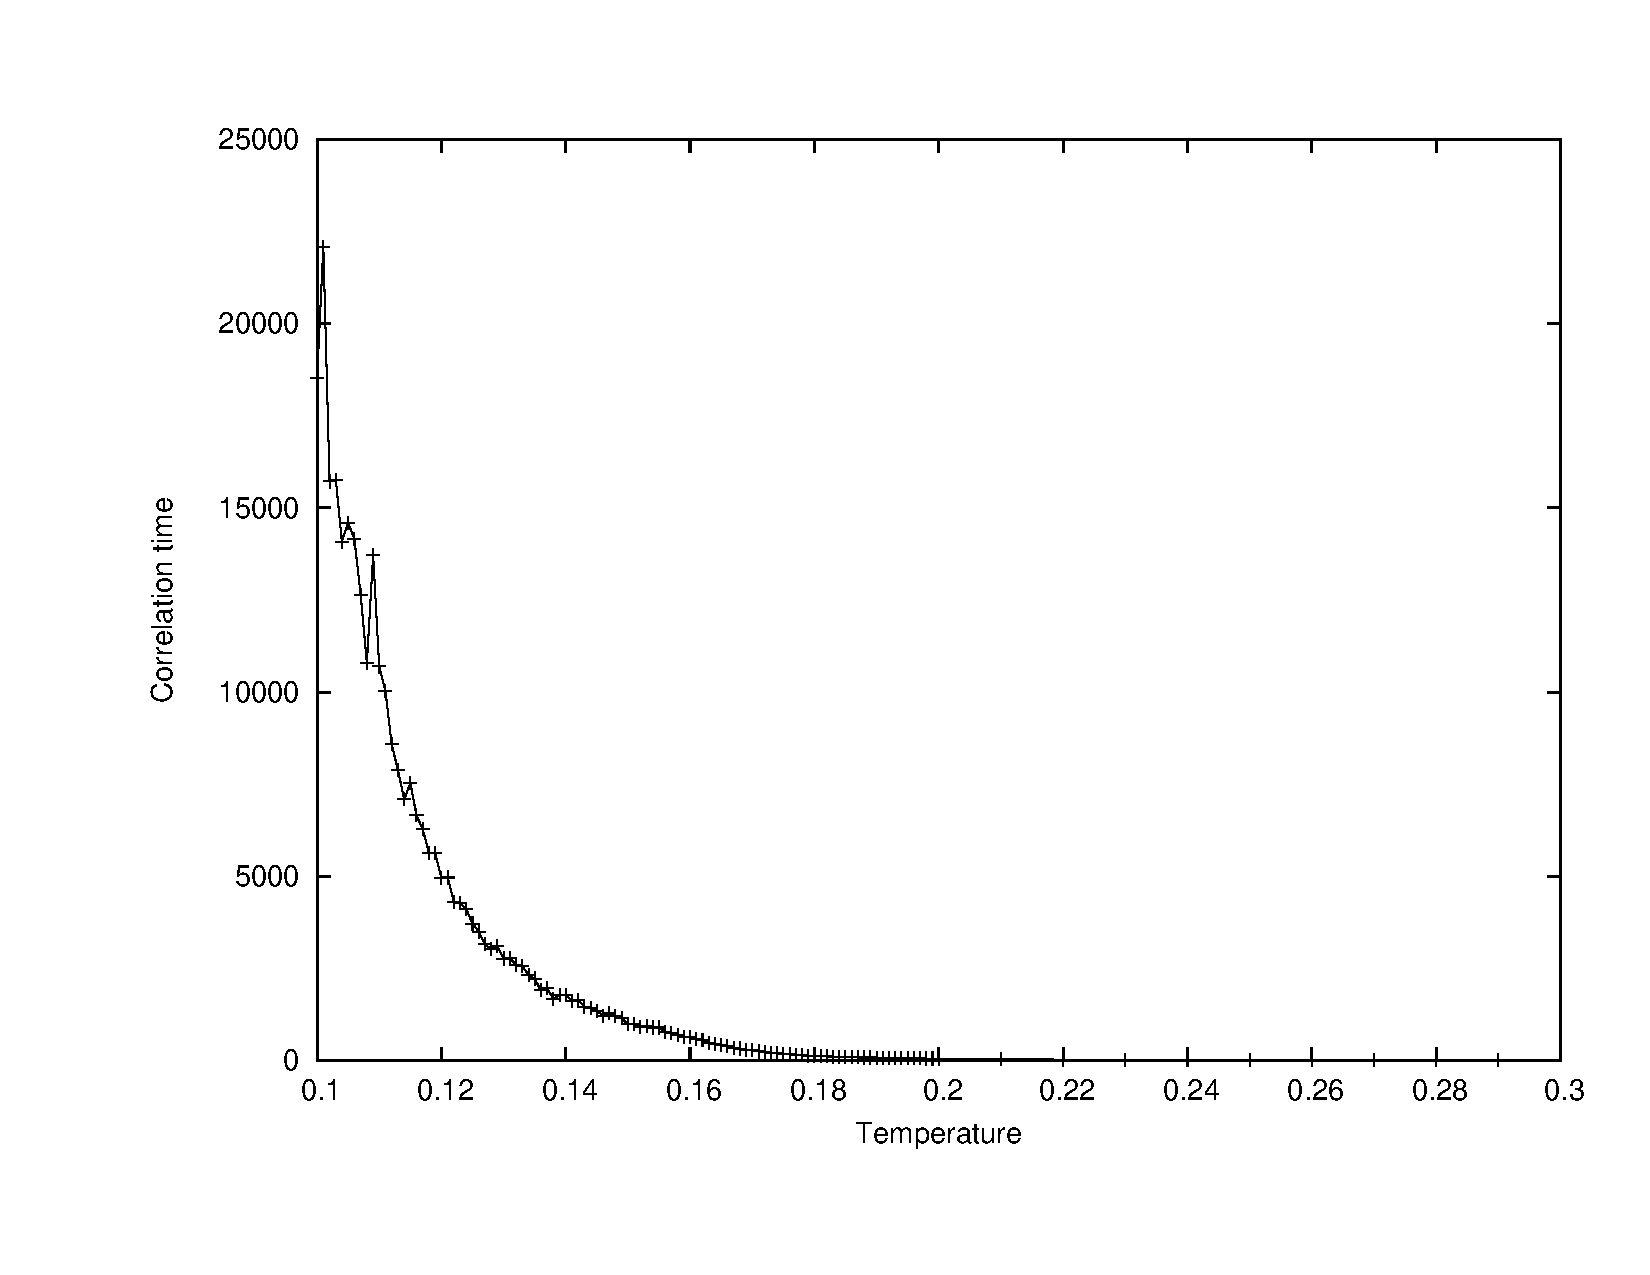
\includegraphics[width=0.5\textwidth, clip, trim = 1.7cm 1.5cm 1cm 1cm]{images/ctimes2}
	\caption{{\footnotesize Gráfico de $\tau(T)$ para o modelo de agregação a 3D, onde T é a temperatura reduzida ($T\equiv\frac{k_b T'}{J}$), para $\rho = 0.2$, com os pontos experimentais ligados por uma linha. A estimativa do tempo foi obtida após equilibrar o sistema com 500000 MCS (passos de monte carlo), calculando a função de autocorrelação (eq.7) e integrando-a, assumindo a forma exponencial já referida.}}
	\label{fig:14}
\end{figure}
\end{frame}

\begin{frame}
\frametitle{\insertsection \\ {\small \insertsubsection}}
\begin{figure}
	\centering
		\includegraphics[width=0.5\textwidth, clip, trim = 1.7cm 1.5cm 1cm 1cm]{images/0.2/c}
	\caption{{\footnotesize Calor específico $c$ para $\rho = 0.2$, calculado após equilibrar o sistema esperando 500000 MCS e fazendo 20 medições da energia a cada 2 tempos de correlação, calculando então as suas flutuações.}}
	\label{fig:15}
\end{figure}
\end{frame}

\begin{frame}
\frametitle{\insertsection \\ {\small \insertsubsection}}
\begin{figure}
	\centering
		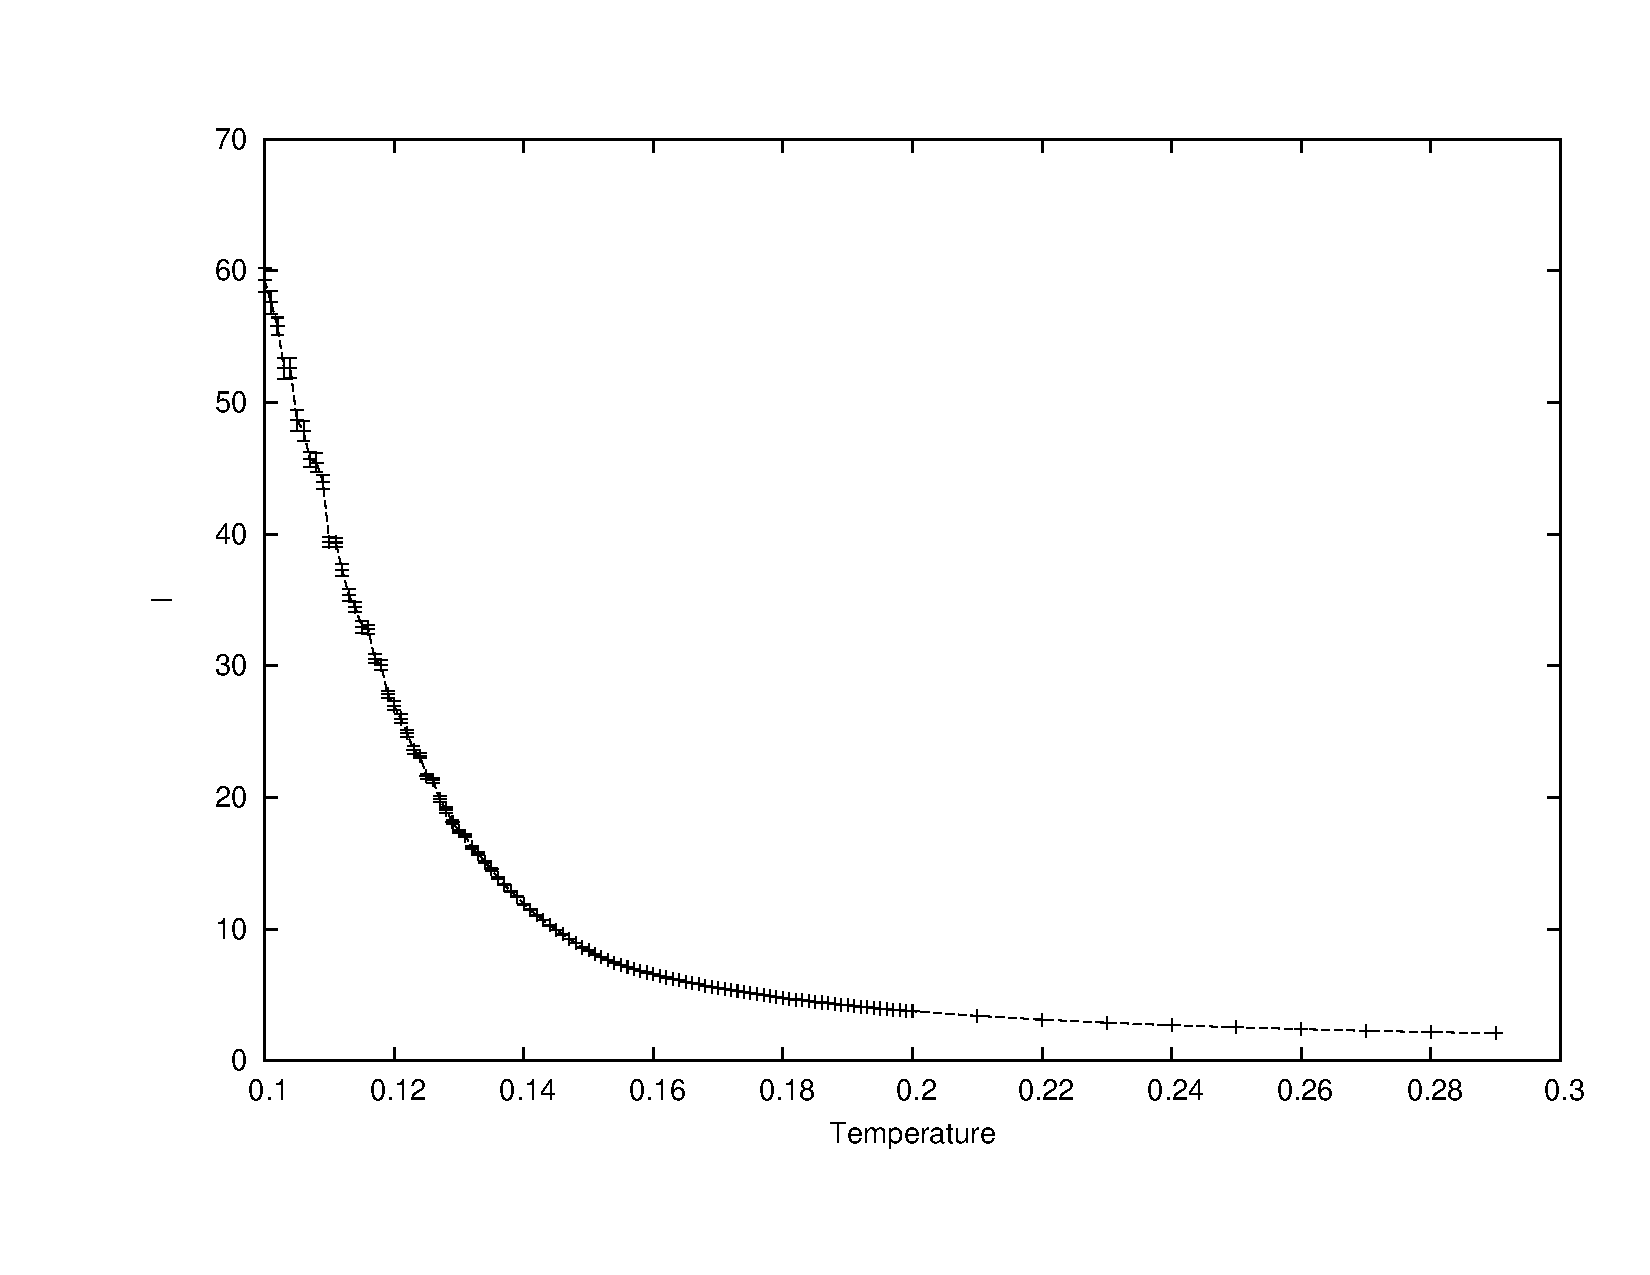
\includegraphics[width=0.5\textwidth, clip, trim = 1.7cm 1.5cm 1cm 1cm]{images/0.2/l}
	\caption{{\footnotesize Comprimento médio das cadeias $\bar{l}$ para $\rho = 0.2$, calculado após equilibrar o sistema esperando 500000 MCS e fazendo 20 medições de $\bar{l}$ a cada 2 tempos de correlação, calculando então a sua média.}}
	\label{fig:16}
\end{figure}
\end{frame}

\begin{frame}
\frametitle{\insertsection \\ {\small \insertsubsection}}
\begin{figure}
	\centering
		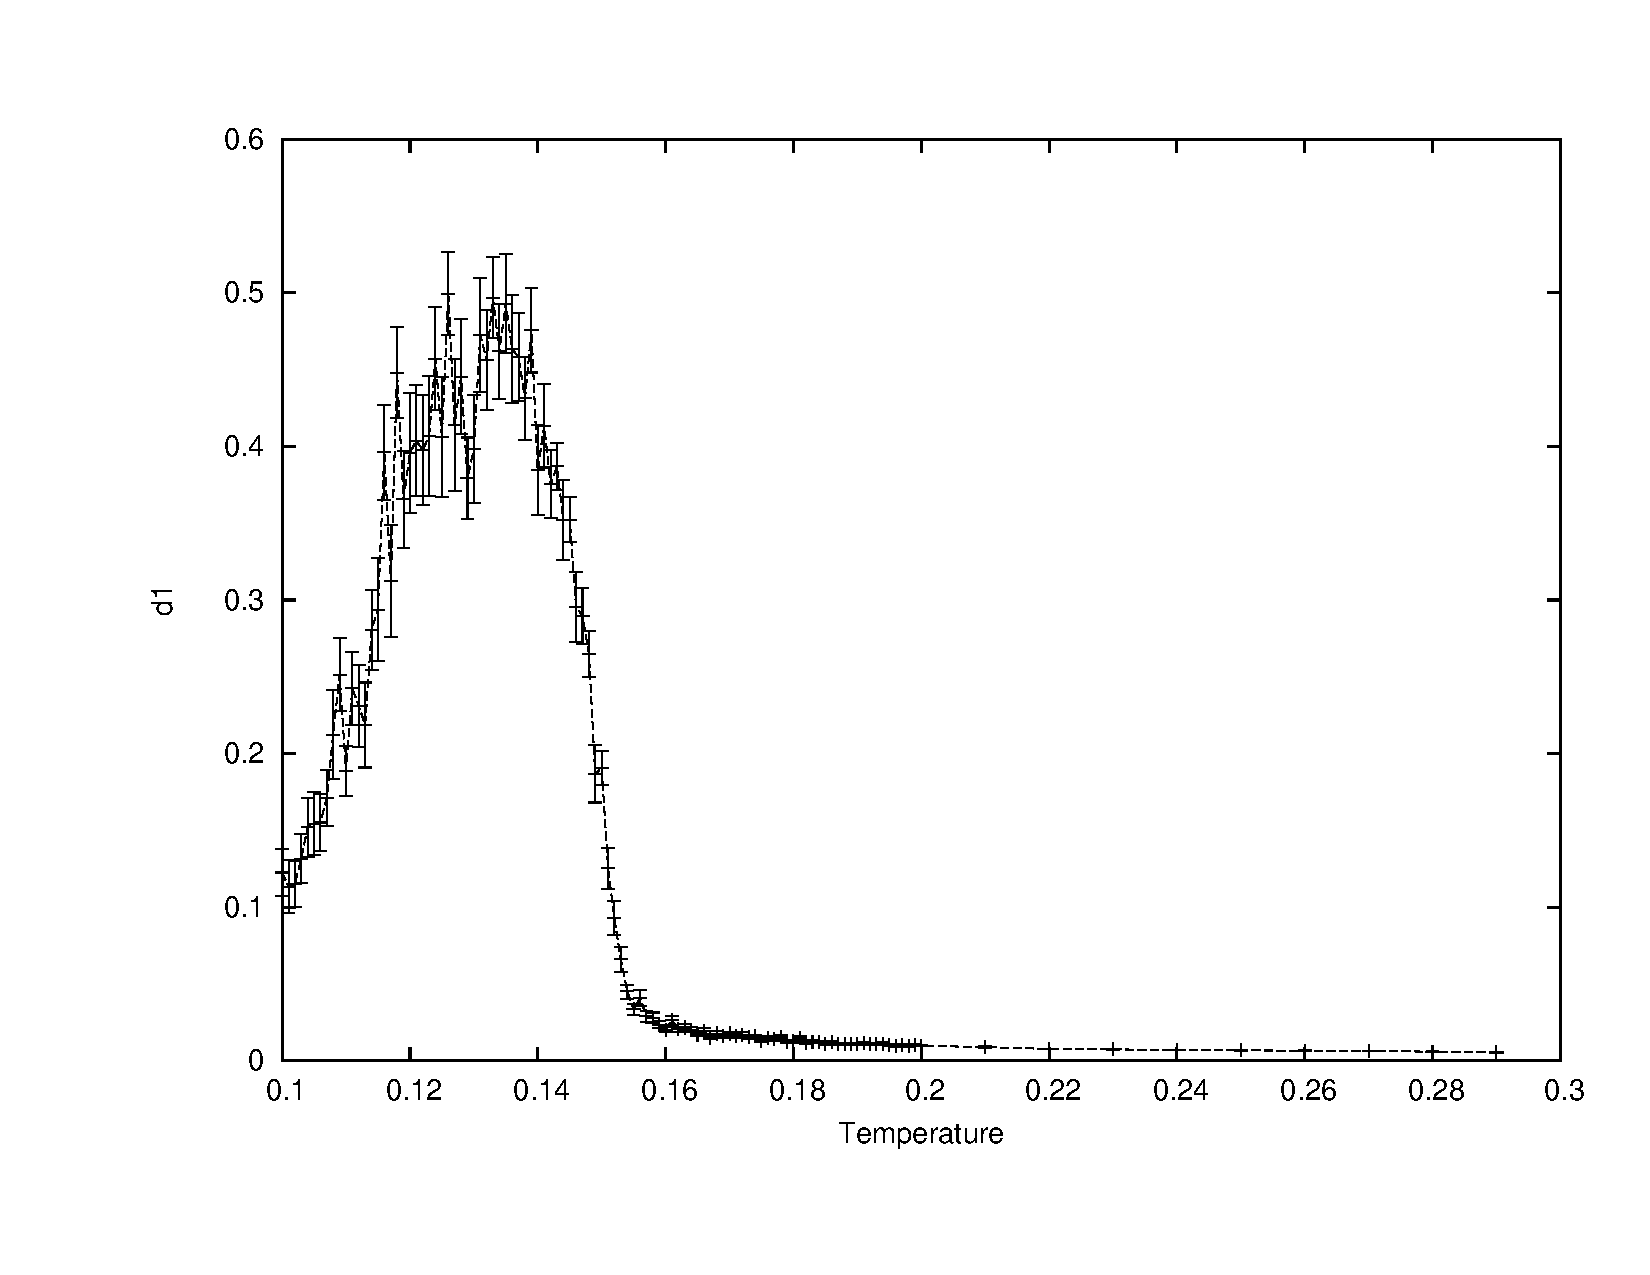
\includegraphics[width=0.5\textwidth, clip, trim = 1.7cm 1.5cm 1cm 1cm]{images/0.2/d1}
	\caption{{\footnotesize Parâmetro de ordem reduzido $|\Delta_1|$ para $\rho = 0.2$, onde $N$ é o número total de partículas. O parâmetro foi calculado após equilibrar o sistema esperando 500000 MCS e fazendo 20 medições de $|\Delta_1|$ a cada 2 tempos de correlação, calculando então a sua média.}}
	\label{fig:17}
\end{figure}
\end{frame}

\begin{frame}
\frametitle{\insertsection \\ {\small \insertsubsection}}
\begin{figure}
	\centering
		\includegraphics[width=0.5\textwidth, clip, trim = 1.7cm 1.5cm 1cm 1cm]{images/0.2/d1f}
	\caption{{\footnotesize Flutuações do parâmetro de ordem reduzido $|\Delta_1|$ para $\rho = 0.2$, calculadas da mesma forma que c. Será em princípio possível ver a transição de fase determinando $T$ para a qual as flutuações tendem para infinito}}
	\label{fig:18}
\end{figure}
\end{frame}

\begin{frame}
\frametitle{\insertsection \\ {\small \insertsubsection}}
\begin{figure}
	\centering
		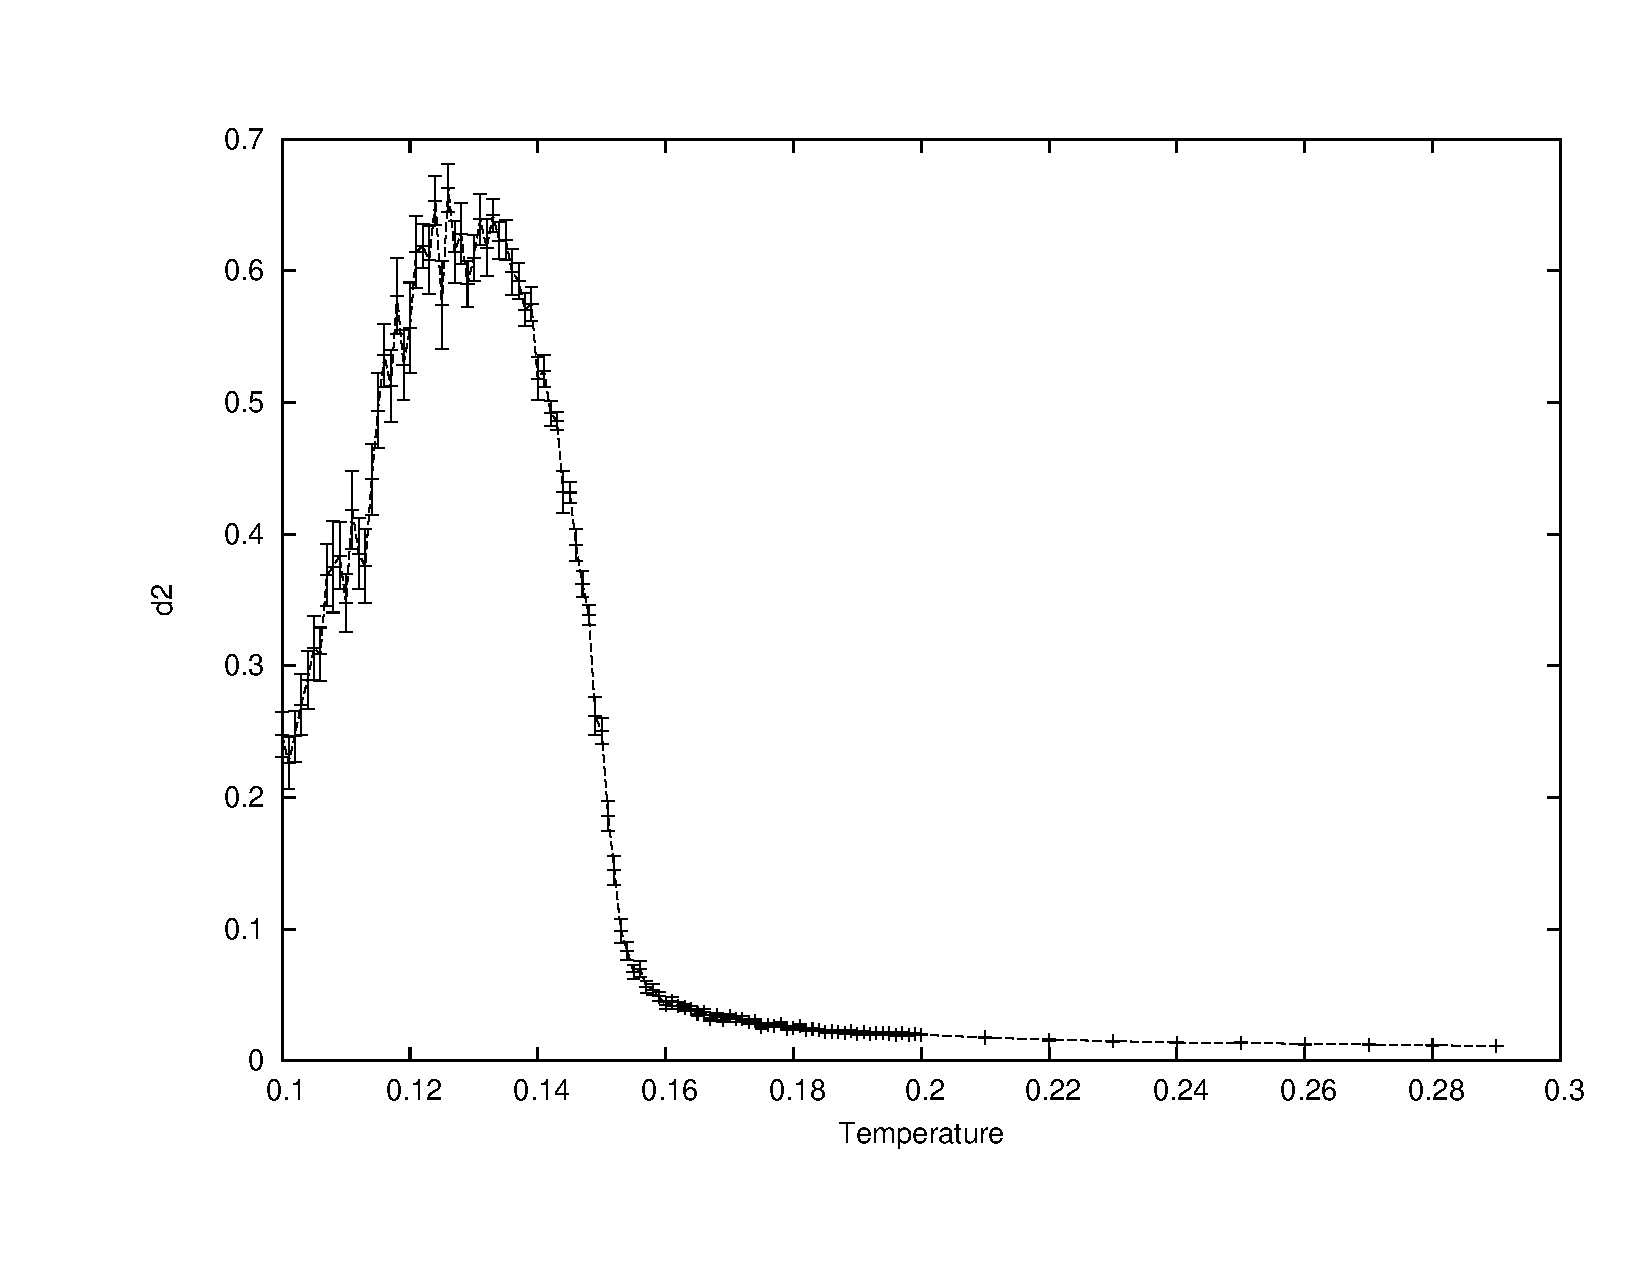
\includegraphics[width=0.5\textwidth, clip, trim = 1.7cm 1.5cm 1cm 1cm]{images/0.2/d2}
	\caption{{\footnotesize Parâmetro de ordem reduzido $|\Delta_2|$ para $\rho = 0.2$, onde $N$ é o número total de partículas. O parâmetro foi calculado após equilibrar o sistema esperando 500000 MCS e fazendo 20 medições de $|\Delta_2|$ a cada 2 tempos de correlação, calculando então a sua média.}}
	\label{fig:19}
\end{figure}
\end{frame}

\begin{frame}
\frametitle{\insertsection \\ {\small \insertsubsection}}
\begin{figure}
	\centering
		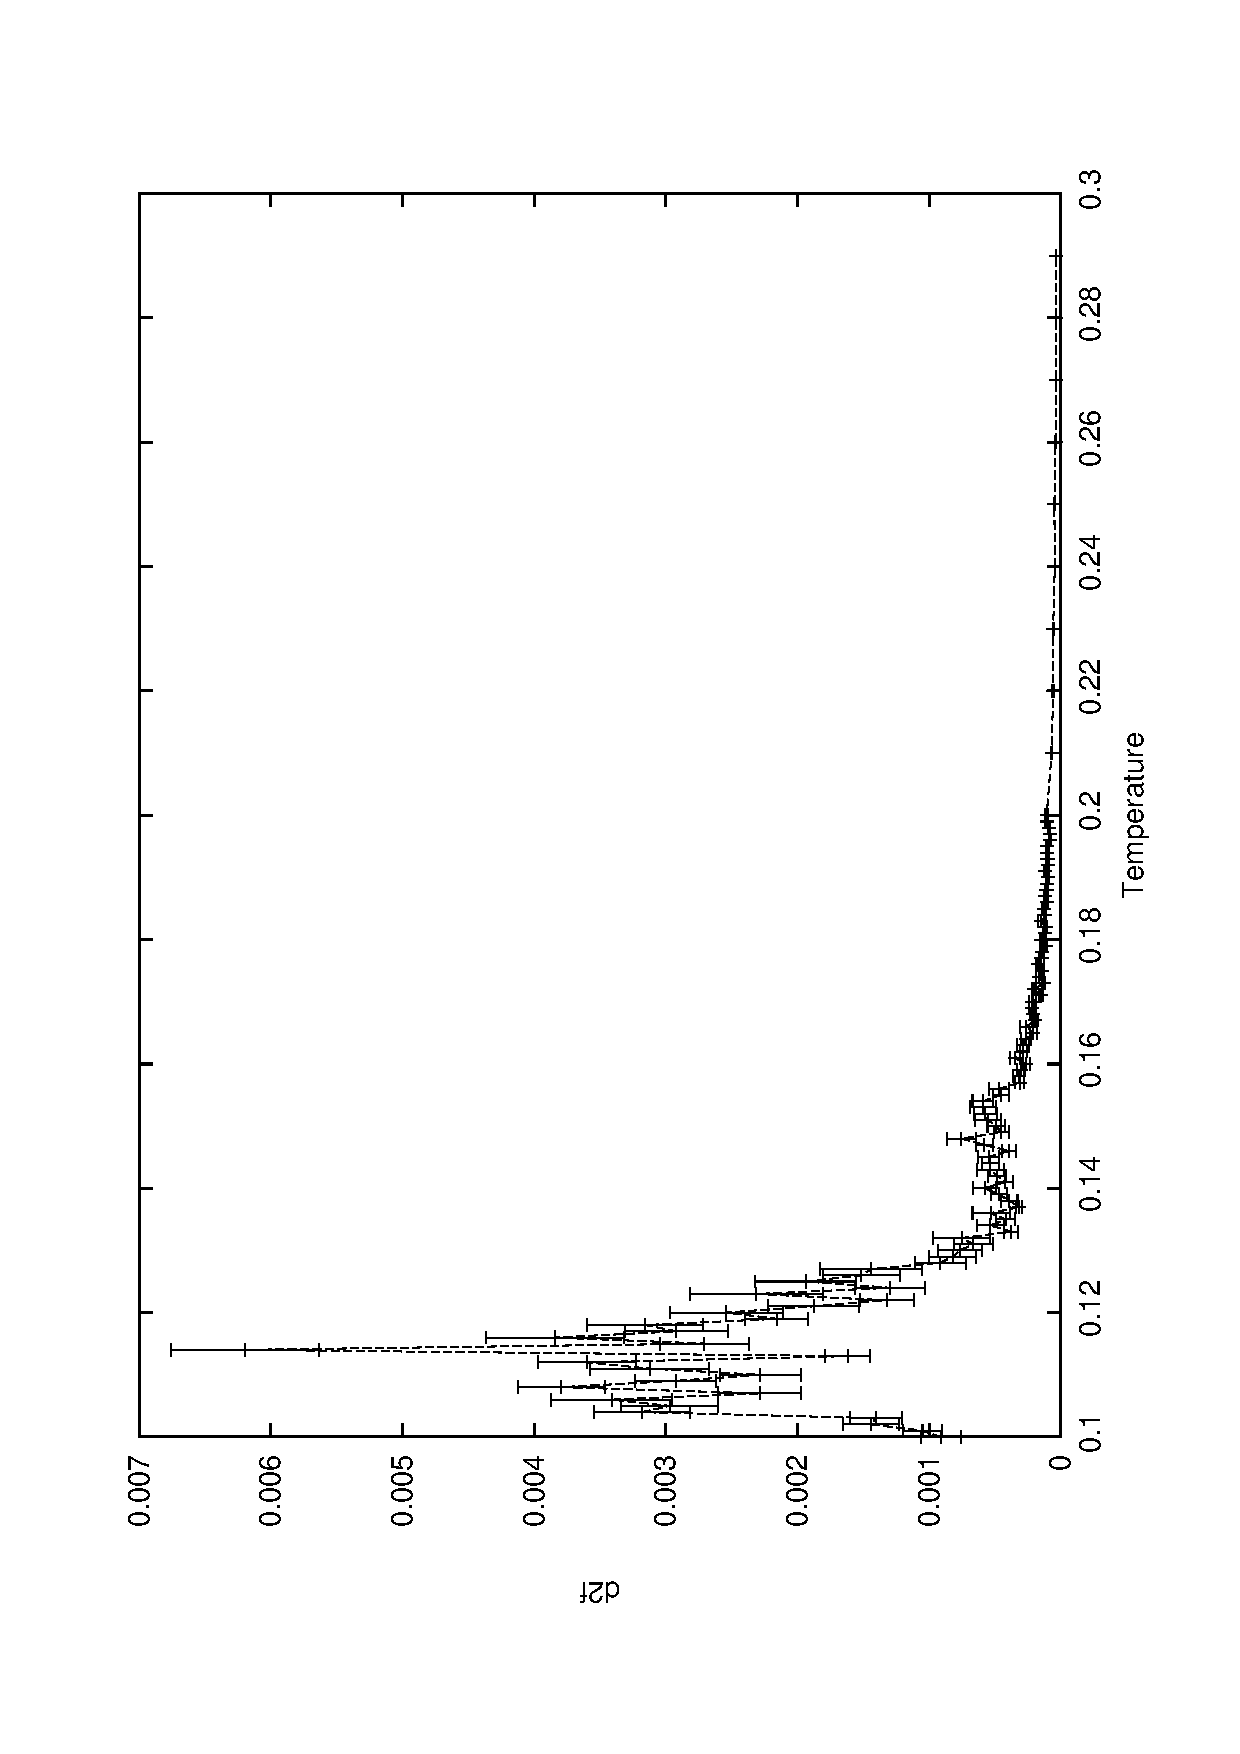
\includegraphics[width=0.5\textwidth, clip, trim = 1.7cm 1.5cm 1cm 1cm]{images/0.2/d2f}
	\caption{{\footnotesize Flutuações do parâmetro de ordem reduzido $|\Delta_2|$ para $\rho = 0.2$, calculadas da mesma forma que c. Será em princípio possível ver a transição de fase determinando $T$ para a qual as flutuações tendem para infinito}}
	\label{fig:20}
\end{figure}
\end{frame}

\subsubsection{Visualização}

\begin{frame}
\frametitle{\insertsection \\ {\small \insertsubsection}}
\begin{figure}
	\centering
		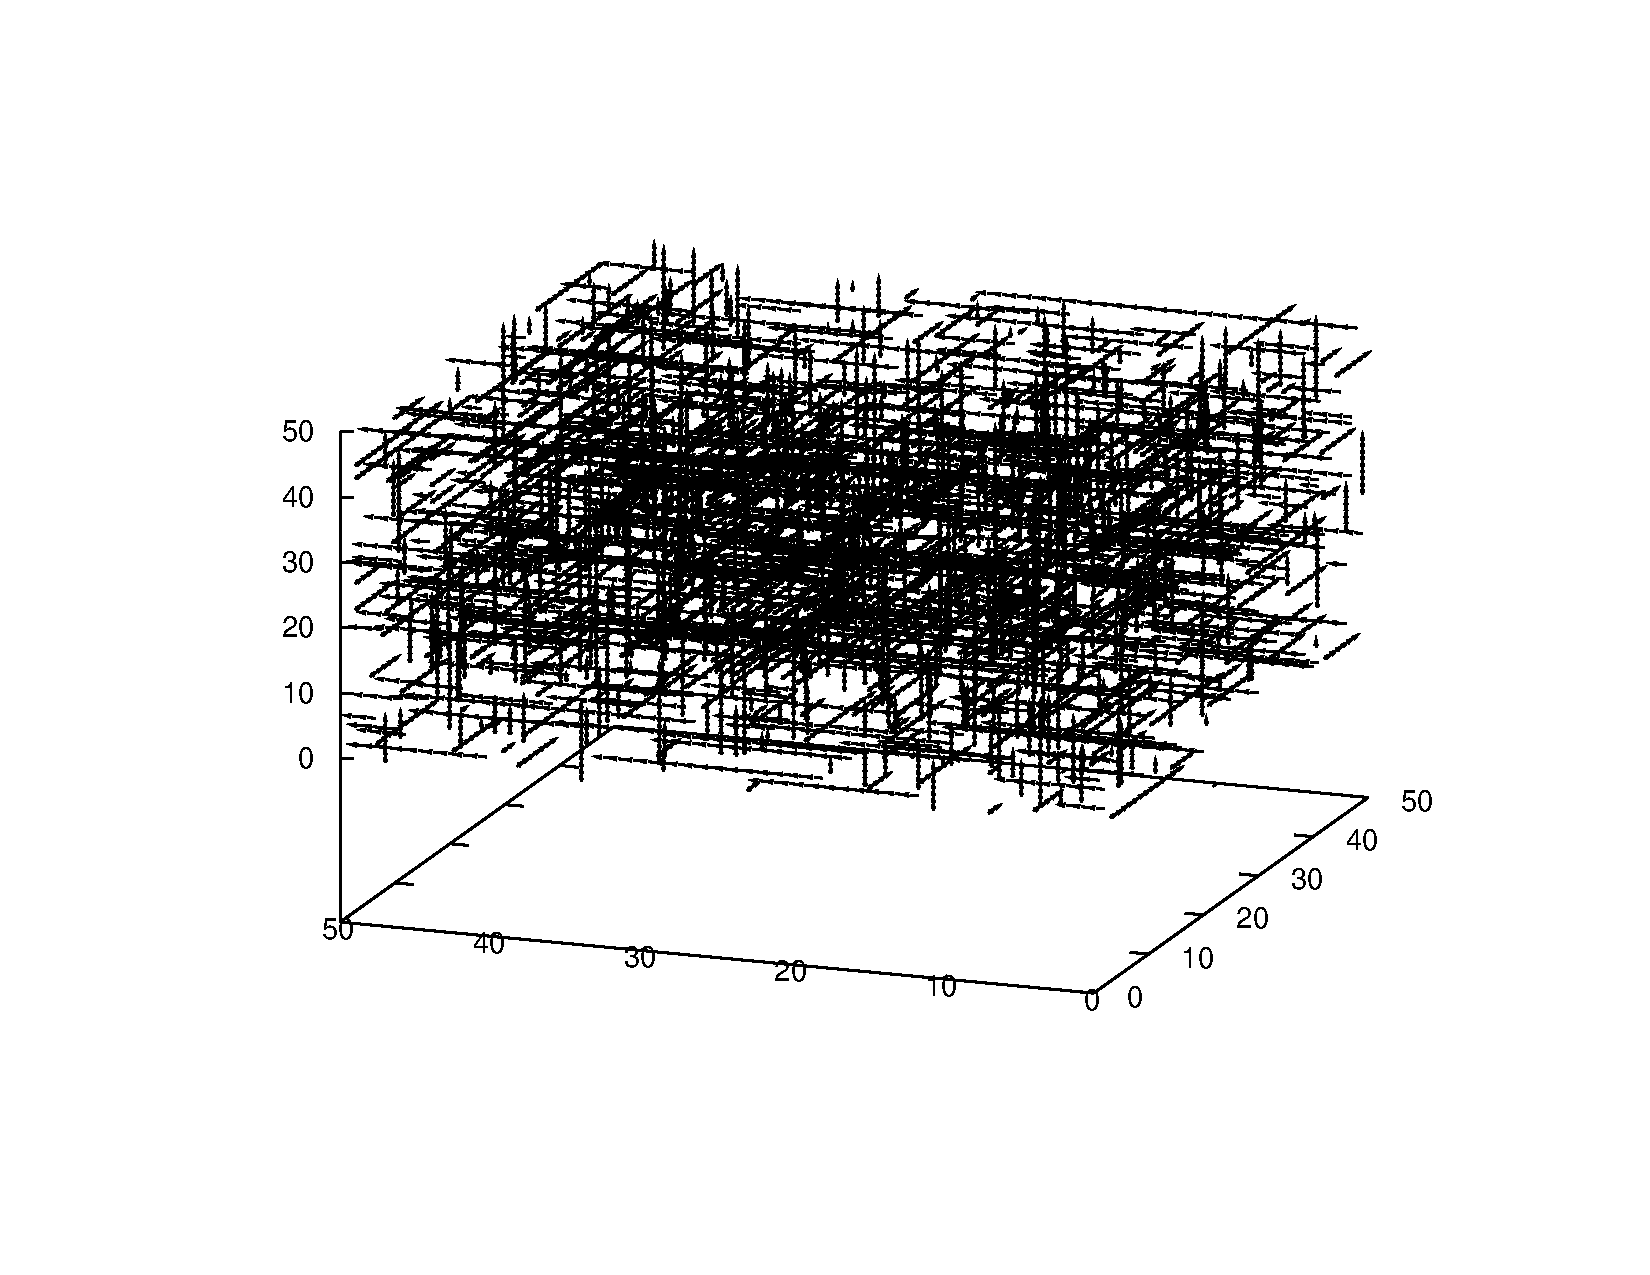
\includegraphics[width=0.5\textwidth, clip, trim = 2.7cm 2.5cm 2cm 2cm]{images/rods3d}
	\caption{{\footnotesize Visualização do sistema 3D numa lattice com L=50 para $T=0.1$, onde as partículas são representadas por vectores orientados pela respectiva direcção. Visualização criada a partir de uma configuração de um sistema equilibrado após 500000 MCS. Apesar da dificuldade de visualização a 3D, para esta densidade pequena é visivel a orientação das partículas em planos, e torna-se óbvio que a dimensão acrescida remove o constrangimento de crescimento para as orientações não predominantes.}}     
	\label{fig:21}
\end{figure}
\end{frame}

\section{Conclusões}
\begin{frame}
\frametitle{\insertsection \\ {\small \insertsubsection}}
\begin{itemize}
\item Modelo de Ising: Pouco interessante do ponto de vista de simulação numérica, permitiu conferir os conceitos básicos.
\item Modelo de agregação linear: permitiu efectuar simulações de sistemas com fenómenos ainda em estudo e pouco conhecidos, como a auto-organização.
\item Reproduziu-se a simulação 2D realizada antes, tendo-se verificado que os resultados concordavam com os obtidos anteriormente.

\end{itemize}
\end{frame}

\begin{frame}
\frametitle{\insertsection \\ {\small \insertsubsection}}
\begin{itemize}
\item Correu-se a simulação em 3 dimensões, com resultados pouco claros.

\item Verificou-se ainda assim a possibilidade de existência de uma transição de fase.

\item Será necessário maior tempo de simulação, e um estudo mais aprofundado do modelo teórico para ter uma ideia mais clara das gamas de parâmetros por volta das quais simular, para confirmar a existência de fenómenos interessantes.
\end{itemize}
\end{frame}

\end{document}
